\chapter{Phrase Indexing and Querying}
\label{chap:phrases}


\section{Motivation and Problem Statement}

Phrases are sequences of multiple words. Phrase queries are such multi-word sequences, typically expressed with quotation marks (e.g., \textsf{``the republic of india''}). In this chapter we deal with the problem of document retrieval for phrase queries-- Given a document collection $D$ and a phrase query $p$, we intend to find all documents $d \in \mathcal{D}$ that literally contain $p$. Our focus in this work is on supporting phrase queries more efficiently.

%% Why is the problem interesting and important?
Phrase queries are supported by all modern search engines and are one
of their most popular among their \emph{advanced} features. Phrases tend to be unambiguous concept markers~\cite{salton1989automatic, croft1991use,lewis1989term} and are known to increase precision in search~\cite{de1999phrase}. Treating a query as a phrase yields documents which are closer to the intended concept like \emph{``six pack''}, \emph{``times square''}, \emph{``hurt locker''}. Even when
unknown to the user, phrase queries can still be implicitly invoked,
for instance, by means of query-segmentation methods~\cite{Hagen:2012fk,Li:2011kx}. Query segmentation refers to pre-retrieval algorithms that automatically introduce phrase queries in the user's input. 

Beyond their usage in search engines, phrase queries increasingly serve as a building block for other applications such as (a)~\emph{entity-oriented search and analytics}~\cite{agrawalCCG:vldb08} (e.g.,~to identify documents that
refer to a specific entity using one of its known labels), (b)~\emph{plagiarism detection}~\cite{Stamatatos:2011uq} (e.g.,~to
identify documents that contain a highly discriminative fragment from
the suspicious document), (c)~\emph{culturomics}~\cite{Michel:ys}
(e.g.,~to identify documents that contain a specific $n$-gram and
compute a frequency time-series from their timestamps).

These applications are also relevant in the context of web archives making phrase queries an important workload type. Search over archives can be extended to use phrase queries by replacing the keyword component in time-travel queries with phrases. Interesting applications which capture entity evolution could potentially use phrase queries to aid entity extraction and tracking over periods of time. 


\subsection{Approach}
%% Why is it hard (E.g., why do naive approaches fail)?
Traditional approaches to phrase-query processing, as outlined in Chapter 2, uses inverted indexes with postings containing positional information. This posting payload captures where words occur in documents has to be maintained to support phrase queries, which leads to indexes that are larger. B\"uttcher et. al.~\cite{Buttcher:2010fk} report a factor of about $4\times$ for the inverted index than those required for keyword queries. Phrase query processing, unlike keyword queries where stop words can be ignored, considers all words in the query. It enforces conjunctive query semantics and also devotes extra processing cycles and memory to ensure that the terms occur in the same order as in the query. Consequently, phrase queries are substantially more expensive to process.

%% Why hasn't it been solved before? (Or, what's wrong with previous
%% proposed solutions? How does mine differ?)

The problem of substring matching, which is at the core of phrase
queries, has been studied extensively by the string-processing
community. However, the solutions developed (e.g.,~suffix
arrays~\cite{Manber:1993vn} and permuterm
indexes~\cite{Ferragina:2010bh}) are designed for main memory and
cannot cope with large-scale document collections such as web archives. Solutions developed
by the infor\-ma\-tion-re\-trie\-val
community~\cite{Transier:2008kx,Williams:2004fk} build on the inverted
index, extending it to index selected multi-word sequences, so-called
\emph{phrases}, in addition to single words. The intuition behind indexing phrases into such an augmented index exploit the fact that word sequences are more selective than words resulting in improved response times. However the selection of which phrases to index has been addressed in a limited manner. Typically phrases having a fixed length are selected based on
heuristics (e.g.,~whether they contain a
stopword~\cite{Chang:2008kx,Williams:2004fk}) or taking into account
characteristics of either the document
collection~\cite{Transier:2008kx} or the workload~\cite{Williams:2004fk}. Indexing additional phrases leads to an increase in index size which brings us to the topic of the natural trade-off between inde size and query performance. All the existing approaches barring~\cite{Transier:2008kx} are agnostic to the index size blowup due to indexing extra phrases and hence do not provide size-based index tuning. 

Once we construct an augmented index as described before we now turn to how queries are processed using such an enriched vocabulary. With the addition of more terms to the lexicon there are multiple choices as to how a phrase query can be processed. As an example, for a query \emph{``we are the champions''} can be processed by \{\emph{``we are''}, \emph{``we are the''}, \emph{``champions''}\} or \{\emph{``we are''}, \emph{``the champions''}\}. A non-optimal choice can sometimes lead to a considerable performance degradation compared to the best choice. In the literature this problem of \emph{phrase-query optimization}, that is, selecting a set of terms to process a given phrase query has been addressed only using greedy heuristics. 

We follow the general approach of augmenting the inverted index
by selected phrases, but our approach differs in several
important aspects. Firstly, it allows for \emph{variable-length phrases} to be indexed while keeping the total index size under a user-specified size budget. We tackle the problem of phrase selection, that is, deciding which phrases should be indexed, by taking into account both the document collection and the workload. The workload indicates how frequent a particular phrase appears in queries. The document collection on the other hand establishes how expensive it is to index a given phrase. We balance both the benefit of usage and storage cost of a phrase to chose a set of phrases which maximize the expected query performance. Secondly, we take a more principled approach to solving the query optimization problem by proposing algorithms which produce an optimal or close-to-optimal set of terms. Note that the ``time-travel'' aspect is orthogonal to the indexing methods proposed in this chapter. In principle one could partition each posting list corresponding to a multi-word sequence for efficiently processing time-travel queries where the keyword component is a phrase query.

%% What are the key components of my approach and results? Also
%% include specific limitations.

\subsection{Contributions} 
We make the following contributions in this chapter.

\begin{enumerate}

\item We introduce the \emph{augmented inverted index} as a generalization of existing approaches.

\item We study the problem of \emph{phrase-query optimization},
  establish its $\mathcal{NP}$-hardness, and describe an exact
  exponential algorithm as well as an $O(log\,n)$-approximation
  algorithm to its solution.

\item We propose two \emph{novel phrase-selection methods} tunable by a
  user-specified space budget that consider characteristics of both
  the document collection and the workload.

\item We carry out an \emph{extensive experimental evaluation} on ClueWeb09 and a
  corpus from The New York Times, as two real-world document
  collections, and entity labels from the YAGO2 knowledge base, as a
  workload, comparing our approach against state-of-the-art
  competitors and establishing its efficiency and effectiveness.
\end{enumerate}

With as little as $5\%$ additional space, our approach improves
phrase-query processing performance by a factor of more than $3\times$
over a standard positional inverted index, thereby considerably
outperforming its competitors.

\subsection{Organization} 

The rest of this chapter unfolds as
follows. Section~\ref{sec:model} introduces our formal model. The
augmented inverted index is described in
Section~\ref{sec:augm-invert-index}. Section~\ref{sec:query-optimization}
deals with optimizing phrase queries. Selecting phrases to be indexed
is the subject of
Section~\ref{sec:phrase-selection}. Section~\ref{sec:exper-eval}
describes our experimental evaluation. We relate our work to existing
prior work in Section~\ref{sec:related-work} and conclude in
Section~\ref{chap:phrases:sec:conclusion}.


\section{Model and Index Organization}
\label{sec:model}

We introduce our formal model and the notation used throughout the rest of the chapter. For easy reference we also recap the notation in Table~\ref{chap:phrases:tab:notation}.

We let $\mathcal{V}$ denote the \emph{vocabulary} of all words. The
\emph{set of all non-empty sequences of words} from this vocabulary is
denoted $\mathcal{V}^{+}$. Given a word sequence
$\mathbf{s} = \seq{s_1,\,\ldots,\,s_n} \in \mathcal{V}^{+}$, we let
$\card{\mathbf{s}} = n$ denote its length. We use $\mathbf{s}[i]$ to
refer to the word $s_i$ at the $i$-th position of $\mathbf{s}$, and
$\mathbf{s}[i..j]$ ($i\le j$) to refer to the word
subsequence~$\seq{s_i,\,\ldots,s_j}$.

\begin{definition}[Position within a sequence]
Given two word sequences $\mathbf{r}$ and $\mathbf{s}$, we let
$pos(\mathbf{r},\mathbf{s})$ denote the set of positions at which
$\mathbf{r}$ occurs in $\mathbf{s}$, formally
$$ %%%
pos(\mathbf{r},\mathbf{s}) = \bigset{1 \le i \le |\mathbf{s}| \:|\: \forall\, 1 \le j \le |\mathbf{r}| : \mathbf{s}[i + j - 1] = \mathbf{r}[j]}\;. %%%
$$ %%%
\end{definition}

For $\mathbf{r} = \seq{a b}$ and $\mathbf{s} = \seq{c a b c a b}$, as
a concrete example, we have $pos(\mathbf{r},\mathbf{s}) = \set{2,5}$.
We say that $\mathbf{s}$ \emph{contains} $\mathbf{r}$ if
$pos(\mathbf{r},\mathbf{s}) \neq \emptyset$. To ease notation, we
treat single words from $\mathcal{V}$ also as word sequences when
convenient. This allows us, for instance, to write
$pos(w, \mathbf{s})$ to refer to the positions at which $w$ occurs in
$\mathbf{s}$.

Until now we operated on versions, however the approaches discussed in this chapter are general enough to be applied to all text collections. Thus for ease of notation we consider a document collection $\mathcal{D}$ of documents $\mathbf{d} \in \mathcal{D}$.
%We let $\mathcal{D}$ denote our \emph{document collection}. 
Each
document $\mathbf{d} \in \mathcal{D}$ is a word sequence from
$\mathcal{V}^{+}$. Since we allow for \emph{duplicate documents},
$\mathcal{D}$ is a bag of word sequences.

We let $\mathcal{W}$ denote our \emph{workload}. Each query
$\mathbf{q} \in \mathcal{W}$ is a word sequence from
$\mathcal{V}^{+}$. Since we allow for \emph{repeated queries},
$\mathcal{W}$ is also a bag of word sequences.

Using our notation, we now define the standard notions of
\emph{document frequency} and \emph{collection frequency}, as common
in Information Retrieval. Let $\mathcal{S}$ be a bag of word sequences
(e.g., the document collection or the workload), we define the
document frequency of the word sequence $\mathbf{r}$, as the total
number of word sequences from $\mathcal{S}$ that contain it, as
$$ %%%
df(\mathbf{r}, \mathcal{S}) = \card{\bigset{\mathbf{s} \in \mathcal{S} \:|\: pos(\mathbf{r},\mathbf{s}) \neq \emptyset }} \;. %%%
$$ %%%
Analogously, its collection frequency, as the total number of
occurrences, is defined as
$$ %%%
cf(\mathbf{r}, \mathcal{S}) = \sum_{\mathbf{s} \in \mathcal{S}} \card{pos(\mathbf{r},\mathbf{s})} \;. %%%
$$ %%%

%
\begin{table}
\centering
\begin{tabular}{ll}
\hline  
\multicolumn{1}{c}{\emph{Notation}} &  \multicolumn{1}{c}{\emph{Description}} \\
\hline
$\mathcal{W}$ & \emph{workload}, a bag of queries\\
$\mathbf{q} \in \mathcal{W}$ & a query\\
$\mathcal{D}$ & collection of documents\\
$\mathbf{d} \in \mathcal{D}$ & a document\\
$\mathcal{V}$ & \emph{vocabulary}, a set of words\\
$\mathbf{w} \in \mathcal{V}$ & a word\\
$\mathcal{V^+}$ & set of non-empty word sequences\\
$\mathbf{s} \in \mathcal{V^+}$ & a word sequence\\
$\mathcal{L} \subseteq \mathcal{V^+}$ & lexicon, the set of indexed word sequences\\
$\mathbf{t} \in \mathcal{D}$ & an indexed word sequence\\
$\mathbf{S}(\mathcal{D})$ & size of the index for the lexicon $\mathcal{D}$ \\
\hline
\end{tabular}

\caption{Notation}\label{chap:phrases:tab:notation}
\end{table}

\section{Indexing Framework}
\label{sec:augm-invert-index}

Having introduced our formal model, we now describe the indexing
framework within which we operate.

We build on the \emph{inverted index} as the most widely-used index
structure in Information Retrieval that forms the backbone of many
real-world systems. The inverted index consists of two components,
namely, a \emph{lexicon} $\mathcal{L}$ of \emph{terms} and
the corresponding \emph{posting lists} that record for each term
information about its occurrences in the document collection. For a
detailed discussion of the inverted index and its efficient
implementation we refer to Chapter~\ref{chap:foundations}.

To support arbitrary phrase queries, an inverted index has to contain
all words from the vocabulary in its lexicon (i.e.,
$\mathcal{V} \subseteq \mathcal{L}$) and record positional information
in its posting lists. Thus, the posting
$\tup{\mathbf{d}_{13},\,\seq{3, 7}}$ found in the posting list for
word $w$ conveys that the word occurs at positions $3$ and $7$ in
document $\mathbf{d}_{13}$. More formally, using our notation, a
posting $\tup{id(\mathbf{d}),\,pos(w,\mathbf{d})}$ for word $w$ and
document $\mathbf{d}$ contains the document's unique identifier
$id(\mathbf{d})$ and the positions $pos(w, \mathbf{d})$ at which the
word occurs.

Query-processing performance for phrase queries on such a
\emph{positional inverted index} tends to be limited, in particular
for phrase queries that contain frequent words (e.g.,
stopwords). Posting lists for frequent terms are long, containing many
postings each of which with many positions therein, rendering them
expensive to read, decompress, and process.

Several authors~\cite{Chang:2008kx,Transier:2008kx,Williams:2004fk}
have proposed, as a remedy, to augment the inverted index by adding
multi-word sequences, so-called \emph{phrases}, to the set of
terms. The lexicon $\mathcal{L}$ of such an \emph{augmented
  inverted index} thus consists of \emph{individual words} alongside
\emph{phrases} (i.e., $\mathcal{L} \subseteq \mathcal{V}^{+}$) as
terms. Phrase selection can be done, for example, taking into account
their selectivity~\cite{Transier:2008kx}, whether they contain a
stopword~\cite{Chang:2008kx,Williams:2004fk}, or based on
part-of-speech tags~\cite{Manning:2008fk}. Our approaches to select
phrases, which take into account both the document collection and the
workload and keep index size within a user-specified space budget, are
detailed in Section~\ref{sec:phrase-selection}.

To process a given phrase query $\mathbf{q}$, a set of terms is
selected from the lexicon $\mathcal{L}$, and the corresponding
posting lists are intersected to identify documents that contain the
phrase. Intersecting of posting lists can be done using
\emph{term-at-a-time} (\textsc{TaaT}) or \emph{document-at-a-time
  query processing} (\textsc{DaaT}). For the former, posting lists are
read one after each other, and bookkeeping is done to keep track of
positions at which the phrase can still occur in candidate
documents. For the latter, posting lists are read in parallel and a
document, when seen in all posting lists at once, is examined for
whether it contains the phrase sought. In both cases, the cost of
processing a phrase query depends on the sizes of posting lists read
and thus the set of terms selected to process the query. 

% \aanand{decide what to do with this piece of text..}
% Existing work
% has addressed this \emph{query-optimization problem}, determining the
% set of terms that should be used to process a given phrase query,
% using greedy heuristics. Our approach to address the problem,
% including its formalization and a study of its hardness, is described
% in Section~\ref{sec:query-optimization}. 

\section{Query Optimization}
\label{sec:query-optimization}

In this section, we describe how a phrase query $\mathbf{q}$ can be
processed using a given augmented inverted index with a concrete
lexicon $\mathcal{L}$. Our objective is thus to determine, \emph{at
query-processing time}, a subset $\mathcal{P} \subseteq \mathcal{L}$ of
terms, further referred to as \emph{query plan}, that can be used to
process $\mathbf{q}$.


%Before we formulate the problem we outline the need for query-optimization by an example. Let us consider the document collection in the example figure~\ref{}. 

To formulate the problem, we first need to capture when a query plan
$\mathcal{P}$ can be used to process a phrase query
$\mathbf{q}$. Intuitively, each word must be covered by at least one
term from $\mathcal{P}$. 

\begin{definition}[Cover of a query]
%$\mathcal{P}$ \emph{covers} $\mathbf{q}$
\begin{eqnarray*}
covers(\mathcal{P}, \mathbf{q}) & \!\!\!=\!\!\! & \forall{\,1 \le i \le \card{\mathbf{q}}} : \exists{\,\mathbf{t} \in \mathcal{P}} : \exists{\,j \in pos(\mathbf{q}[i], \mathbf{t})} : \\
& & \forall{\,1 \le k \le \card{\mathbf{t}} : \mathbf{q}[i - j + k] = \mathbf{t}[k]}
\end{eqnarray*}
\end{definition}

Consider a lexicon $$\mathcal{L} = \bigset{ \seq{a},\seq{b},\seq{c},\seq{d}, \seq{a b}, \seq{b c}, \seq{c d}}.$$ The phrase query $\mathbf{q} = \seq{a b c}$, for instance, can be
processed using $\bigset{\seq{a b}, \seq{b c}}$ but not
$\bigset{\seq{a b}, \seq{c d}}$. 

Without the augmented index, each query term was covered by exactly one term. With the augmented index there are more choices to process each query term. The choices for covering $b$ are $\seq{b}, \seq{a b}$ and $\seq{b c}$. Multiple choices for processing each position in the query leads to combinatorial choices for covering the query. In order to chose the best query plan we would need to quantify the cost of each query cover.

As detailed above, in Section~\ref{sec:augm-invert-index}, different ways of processing a phrase query (i.e.,~\textsc{TaaT} vs. \textsc{DaaT}) exist. In the worst case, regardless of which query-processing method is employed,
all posting lists have to be read in their entirety. We model the cost
of a query plan $\mathcal{P}$ as the total number of postings that has
to be read
$$
c(\mathcal{P}) = \sum_{t\in\mathcal{P}} df(t, C)\;.
$$

While posting sizes are not uniform (e.g., due to compression and
varying numbers of contained positions), which may suggest collection
frequency as a more accurate cost measure, we found little difference
in practice and thus, for simplicity, stick to document frequency in
this work. This is in line with~\cite{macdonald2012learning}, who found that aggregate posting-list lengths is the single feature most correlated with response time for full query evaluation, as required for phrase queries, which also do not permit dynamic pruning.

Prior work in~\cite{Transier:2008kx,Williams:2004fk} use cost-based heuristics to determine a valid query plan. A candidate set of sequences $\rho$ is first determined which are both present in the query as well as the lexicon, i.e.,
$$
 \rho ~=~ \bigset{ r ~|~ r \in \mathcal{L} \,\wedge\, pos(r,q) \neq \phi}.
$$

Candidates are then greedily chosen from $R$ in the order of ascending $df$ values until the entire query is covered. In every round the best candidate which overlaps with the uncovered regions of the query is chosen. However, such a heuristic algorithm might not yield an optimal plan. We illustrate this with an example. Consider a lexicon $\mathcal{L}$ with the following $df$ values

\begin{tabular}{l|r}
   &\\
   &~~ $df(\seq{a b}) = 10$ \\
  $\mathcal{L} = \bigset{ \seq{a},\seq{b},\seq{c},\seq{d}, \seq{a b}, \seq{b c}, \seq{c d}}$ ~&~~ $df(\seq{a b}) = 10$\\
   &~~ $df(\seq{c d}) = 60$\\
   \end{tabular}
$$
$$
A phrase query $\mathbf{q} = \seq{a b c d}$ evaluated according to the greedy heuristic above yield the following plan -- $GRD = \bigset{\seq{a b}, \seq{b c}, \seq{c d}}$ -- with an cost $c(GRD) = 120$. It is easy to see that the optimal cover $OPT$ of this query is $OPT = \bigset{\seq{a b}, \seq{c d}}$ with an cost $c(OPT) = 70$. 

Theoretically, one can construct a worst case scenario which can lead to arbitrary degradation of performance. As an example let there be a query $q = \seq{q_1 \cdots q_m}$. Assuming that only bi-grams are indexed and the distribution of $df$ values are such that $df(\seq{q_i q_{i+1}}) \,<\, df(\seq{q_{i+1} q_{i+2}})$. The cost of the query plan using the greedy heuristic is $\sum_{1 \leq i < m}df(\seq{q_i q_{i+1}})$.

We take a more principled approach and model the query-optimization as an optimization problem. Assembling the above definitions of coverage and cost, we now formally
define the problem of finding a cost-minimal query plan $\mathcal{P}$
for a phrase query $\mathbf{q}$ and lexicon~$\mathcal{L}$ as the
following $\mathcal{NP}$-hard optimization problem
\begin{definition}{\textsc{Phrase-Query Optimization}}
$$
  \argmin{\mathcal{P} \subseteq \mathcal{L}} c(\mathcal{P}) \quad\mbox{s.t.}\quad covers(\mathcal{P},\mathbf{q}) \;.
$$


\end{definition}
\begin{theorem}{}
\label{thm:PQONP} 
 \textsc{Phrase-Query Optimization} is $\mathcal{NP}$-hard.
\end{theorem} 

\begin{proof}{} Our proof closely follows
  Neraud~\cite{Neraud:1990fk}, who establishes that deciding whether a
  given set of strings is elementary is $\mathcal{NP}$-complete. We
  show through a reduction from \textsc{Vertex Cover} that the
  decision variant of \textsc{Phrase-Query Optimization} (i.e.,
  whether a $\mathcal{P}$ with $c(\mathcal{P}) \le \tau$
  exists) is $\mathcal{NP}$-complete, from which our claim follows.

  Let $G(V,E)$ be an undirected graph with vertices $V$ and edges
  $E$. We assume that there are no isolated vertices, i.e., each
  vertex has at least one incident edge. \textsc{Vertex Cover} asks
  whether there exists a subset of vertices $VC \subseteq V$ having
  cardinality $\card{VC} \le k$, so that
  $$\forall\,(u,v) \in E \::\: u \in VC \vee v \in VC,$$ that is, for
  each edge one of its connected vertices is in the vertex cover.

  We obtain an instance of \textsc{Phrase-Query Optimization} from
  $G(V,E)$ as follows:
  \begin{itemize}
  \item $\mathcal{V} = V \cup E$ -- we introduce a word to the
    vocabulary for each vertex ($v$) and edge ($\overline{uv}$) in the
    graph;

  \item $\mathbf{q} = \!\!\biguplus\limits_{(u,v) \in E} u\,\,\overline{uv}\,\,v$
    -- we obtain the query $\mathbf{q}$ as a concatenation of all edge
    words $\overline{uv}$ bracketed by the words of their source ($u$)
    and target ($v$);

  \item $\mathcal{D} = \bigset{\mathbf{q}}$ -- the document collection
    contains only a single document that equals our query;

  \item
    $\mathcal{L} = \mathcal{V} \quad\cup
    \bigcup\limits_{(u,v) \in E}\bigset{\seq{u\,\,\overline{uv}}}
    \quad\cup \bigcup\limits_{(u,v) \in
      E}\bigset{\seq{\overline{uv}\,\,v}}$
    -- each vertex word ($v$) and edge word ($\overline{uv}$) is
    indexed as well as each combination of edge and source
    ($u\,\overline{uv}$) and edge and target ($\overline{uv}\,v$).
  \end{itemize}
  This can be done in polynomial time and space. Note that, by
  construction, $\forall{\,\mathbf{t} \in \mathcal{L}} \::\: df(\mathbf{t},
  \mathcal{D}) = 1$
  holds. We now show that $G(V,E)$ has a vertex cover with cardinality
  $\card{VC} \le k$ iff there is a query plan $\mathcal{P}$ with
  $c(\mathcal{P}) \le k + \card{E}$.
  
  ($\Rightarrow$) Observe that $VC$ contains at least one of $u$ or
  $v$ for each $u\,\,\overline{uv}\,\,v$ from the query, incurring a
  cost of $\card{VC} \le k$. We can complement this to obtain a query
  plan $\mathcal{P}$ by adding exactly one term
  ($\seq{\overline{uv}}$, $\seq{u\,\overline{uv}}$, or
  $\seq{\overline{uv}\,v}$) for each $u\,\,\overline{uv}\,\,v$ from
  the query, incurring a cost of $\card{E}$. Thus,
  $c(\mathcal{P}) \le k + \card{E}$ holds.

  ($\Leftarrow$) Observe that $\mathcal{P}$ must cover each
  $u\,\,\overline{uv}\,\,v$ from the query in one of four ways:
  (i)~$\seq{u} \seq{\overline{uv}} \seq{v}$,
  (ii)~$\seq{u} \seq{\overline{uv}\,v}$,
  (iii)~$\seq{u\,\overline{uv}} \seq{v}$
  (iv)~$\seq{u\,\overline{uv}} \seq{\overline{uv}\,v}$. Whenever a
  $u\,\,\overline{uv}\,\,v$ from the query is covered as
  $\seq{u\,\overline{uv}} \seq{\overline{uv}\,v}$, we replace
  $\seq{u\,\overline{uv}}$ by $\seq{u}$, thus reducing case (iv) to
  case (ii). We refer to the query plan thus obtained as
  $\mathcal{P'}$. Note that $c(\mathcal{P}') \le c(\mathcal{P})$,
  since all terms have the same cost. $\mathcal{P}'$ contains exactly
  one term ($\seq{\overline{uv}}$, $\seq{u\,\overline{uv}}$, or
  $\seq{\overline{uv}\,v}$) for each $u\,\,\overline{uv}\,\,v$ from
  the query, incurring a cost of $\card{E}$. Let $VC$ be the set of
  vertices whose words are contained in $\mathcal{P}'$. We can thus
  write $c(\mathcal{P}') = \card{VC} + \card{E}$. $VC$ is a vertex
  cover, since after eliminating case (iv), each
  $u\,\,\overline{uv}\,\,v$ from the query is covered using either
  $\seq{u}$ or $\seq{v}$. Thus,
  $c(\mathcal{P}') = \card{VC} + \card{E} \le c(\mathcal{P}) \le
  \card{E} + k \Rightarrow \card{VC} \le k$.
\end{proof}

\subsection{Optimal Solution}
\label{sec:optimal-solution}

If an optimal query plan $\mathcal{P}^*$ exists, so that every term
therein occurs exactly once in the query, we can determine an optimal
query plan using dynamic programming based on the recurrence
\begin{equation*}
\textsc{Opt}(i) \!=\!
\left\{\begin{array}{c@{\,:\,\,}c}
 df(\mathbf{q}[1..i], \mathcal{D}) & \mathbf{q}[1..i] \in \mathcal{L}\\
 \!\!\simplemin{j<i}{\!\left(\textsc{Opt}(j) + \!\!\!\!\simplemin{\stackrel{k \le j+1 \, \wedge}{\mathbf{q}[k..i] \in \mathcal{L}}}{\!\!\!\!df(\mathbf{q}[k..i], \mathcal{D})} \right)} & \mbox{otherwise}
 \end{array}\right.
\end{equation*}
in time $\mathcal{O}(n^2)$ and space $\mathcal{O}(n)$ where
$\card{\mathbf{q}} = n$. $\textsc{Opt}(i)$ denotes the cost of an
optimal solution to the prefix subproblem $\mathbf{q}[1..i]$ -- once
the dynamic-programming table has been populated, an optimal query
plan can be constructed by means of backtracking. In the first case,
the prefix subproblem can be covered using a single term. In the
second case, the optimal solution combines an optimal solution to a
smaller prefix subproblem, which is the optimal substructure inherent
to dynamic programming, with a single term that covers the remaining
suffix.
\begin{theorem}{}
 \label{thm:DP} 
 If there is an optimal query plan $\mathcal{P}^*$ for a phrase query
 $\mathbf{q}$ such that
 $$
  \forall{\,\mathbf{t} \in \mathcal{P}^*} \::\: \card{pos(\mathbf{t}, \mathbf{q})} = 1\;,
 $$  
 then $c(\mathcal{P}^*) = \textsc{Opt}(\card{\mathbf{q}})$, that is,
 an optimal solution can be determined using the recurrence
 $\textsc{Opt}$.
\end{theorem}

\begin{proof}{}
  Observe that Theorem~\ref{thm:DP} is a special case of
  Theorem~\ref{thm:EEA} for $\mathcal{F}=\emptyset$. We therefore only
  prove the more general Theorem~\ref{thm:EEA}.
\end{proof}

 It entails that we can efficiently determine optimal query plans for phrase
queries that do not contain any repeated words.
\begin{corollary}{}
  \label{cor:NR}
  We can compute an optimal query plan for a phrase query $\mathbf{q}$
  in polynomial time and space, if 
  $$
  \forall{\,1 \le i \le \card{\mathbf{q}}} \::\: \card{pos(\mathbf{q}[i], \mathbf{q})} = 1 \;.
  $$
\end{corollary}
In practice this special case is important: We found that about $99\%$
of phrase queries in our workload do not contain any repeated words,
as detailed in Section~\ref{sec:exper-eval}.

\paragraph{Algorithm}

We present the algorithm which efficiently implements the recurrence relation. The input to the algorithm are the query $\mathbf{q}$ and the lexicon $\mathcal{L}$. A set of candidate word sequences $\mathcal{R}$ is constructed such that
$
  Cand = \bigset{ \mathbf{s} \in \mathcal{L} \::\: \card{pos(\mathbf{s}, \mathbf{q})} > 1}
$. Let us denote the begin and of a sequence $\mathbf{s} \in \mathcal{R}$ as $begin(\mathbf{s})$ and end of the sequence as $end(\mathbf{s})$. For example, $begin(\mathbf{q}) = 0$ and $end(\mathbf{q}) = |\mathbf{s}|-1$. The cost of each sequence $\mathbf{s}$ is denoted by $c(\mathbf{s}) = df(\mathbf{s})$.

We note that the sequences have a anti-monotonocity property on their costs as stated below which we utilize to prune the candidate set of sequences.
\begin{lemma}[Cost-anti monotonicity of sequences]
For a pair of sequences $r$ and $s$, it holds
\begin{equation*}
  |pos(r,s)| > 1 \,\,\,\implies \,\,\,df(r) \geq df(s).
\end{equation*}
\end{lemma}
\begin{proof}{}
  Every occurence of a sequence of $s$ in the collection is also an occurence of $r$.
\end{proof}

We exploit the cost-anti monotonicity property of sequences to eliminate sequences in $\mathcal{R}$ which are substrings of other candidate sequences. If the entire query $\mathbf{q}$ is indexed, i.e, $\mathbf{q} \in \mathcal{L}$, then all the remaining candidates are pruned out and we can terminate immediately.

After the pruning step it is easy to see that each there can be only one sequence which begins from or ends at any given position $0 \leq i < |\mathbf{q}|$ in the query. We organize the remaining sequences into a list $\mathcal{I}$ ordered by their increasing end positions $end(\mathbf{s})$, i.e,
$$
  \mathcal{I} = \langle \, \mathbf{s}_i\,  \rangle\,: \, \mathbf{s}_i \in Cand \,\, \wedge\,\, \nexists \mathbf{s}_j \in \mathcal{I}, \,\, pos(\mathbf{s}_i, \mathbf{s}_j) > 0  \,\,\, \wedge \,\,\, end(s_i) \leq end(s_{i+1}).
$$ 

Dynamic programming proceeds by computing optimal solutions $\textsc{Opt}(i)$ to the prefix subproblems $\mathbf{q}[1...i]$, i.e, optimal cost of covering the first $i$ positions of $\mathbf(q)$. Since $\mathcal{I}$ is ordered ends of sequences, in every iteration we consider a new sequence $\mathbf{s}$ which increases the problem size to $\mathbf{q}(1...end(\mathbf{s}))$. We compute $\textsc{Opt}(end(\mathbf{s}))$ by trying to minimize $\textsc{Opt}(j) + c(\mathbf{s})$ for $1<j<end(\mathbf{s})$. We also ensure that the new solution $\textsc{Opt}(end(\mathbf{s}))$ also a cover for $\mathbf{q}(1...end(\mathbf{s}))$. Thus $\mathbf{s})$ is the last sequence in the optimal solution for the $\mathbf{q}(1...end(\mathbf{s}))$. We store these last sequences for optimal subproblems in a queue $Q$. Thus each sequence $\mathbf{t}$ in a queue encodes the solution to the subproblem $\mathbf{q}(1...end(\mathbf{t}))$, i.e., $\textsc{Opt}(end(\mathbf{t}))$. Since each element of $Q$ is the last sequence in their respective subproblems, the future sequences considered only have to check overlaps with the sequences in the queue to ensure that the subproblems that they represent are covered. We let $last(Q)$ denote the sequence at the end of the queue or the last sequence added. 

%The sequence $\mathbf{s}$ with an end $i = end(\mathbf{s})$, as discussed earlier, is associated with the optimal solution $\textsc{Opt}(i)$ and is appended at the tail of the queue. 

We establish an invariance in plan cost, i.e., $\textsc{Opt}(i+1) > \textsc{Opt}(i)$ over the sequences in $Q$. Thus if an incoming sequence computes with end $i$ has $\textsc{Opt}(i)$ greater than earlier values of $\textsc{Opt}$ in the queue, then those sequences are removed until the invariance is established. After determining the optimal solution for which $\mathbf{s}$ is the last sequence, and maintaining the invariance by pruning out sequences in $Q$, $\mathbf{s}$ is appended to the end of $Q$.

 After we have exhausted all input values from $\mathcal{I}$, as a final step, we backtrack from the last sequence representing $\textsc{Opt}(|\mathbf{q}|)$ to construct the plan with the minimum cost (c.f. lines 18-21). Then invariance improves the efficiency of the algorithm by  decreasing the number of comparisons (i) while determining a feasible cover (line 7) and (ii) while backtracking for the determination of the final plan.


\begin{algorithm}[htb!]
%\LinesNumbered
  \KwIn{Phrase query $\mathbf{q}$, lexicon $\mathcal{L}$}
  \KwOut{Cost $optCost$ of optimal query plan}

\Begin{

  $Cand = \bigset{ \mathbf{s} \in \mathcal{L} \::\: \card{pos(\mathbf{s}, \mathbf{q})} > 0}$\;

$
  \mathcal{I} = \langle \, \mathbf{s}_i\,  \rangle\,: \, \mathbf{s}_i \in Cand \,\, \wedge\,\, \nexists \mathbf{s}_j \in \mathcal{I}, \,\, pos(\mathbf{s}_i, \mathbf{s}_j) > 0  \,\,\, \wedge \,\,\, end(s_i) \leq end(s_{i+1})
$\;

$Q \longleftarrow \langle i_1 \rangle$\; //$ Q$ is the queue of processed sequences.

\BlankLine
\BlankLine
\BlankLine


\For{$\mathbf{s} \in \mathcal{I}$}{
  %$i_{min} = \argmin{i_k \in Q \,\,\wedge \,\, p_f(i_j) \in [ p_f(i_k), p_l(i_k) ]}{\left( p_l(i_k) - p_f(i_j) \right)} $\;
  
  $i_{min} = \argmin{i_k \in Q \,\,\wedge \,\, begin(i_k) \leq begin(\mathbf{s}) \leq begin(i_k)}{\left( end(i_k) - begin(\mathbf{s}) \right)} $\;
  

  \BlankLine
  \BlankLine

  // $i_{min}$ is the sequence with the minimum intersection with $i_j$.
  \If{$i_{min} = \emptyset$} {
          $\textsc{Opt}(i_{min}) = 0$ \;
  }

  
  $\textsc{Opt}(end(\mathbf{s})) = \textsc{Opt}(i_{min}) + c(\mathbf{s})$\;
    \BlankLine
    \BlankLine

  
      // Preserving increasing score order in Q
       
       \While{$\textsc{Opt}(end(Q.last)) > \textsc{Opt}(end(\mathbf{s}))$}{
          $removeLastSequence(Q)$\;
       }
       $AppendInterval(\mathbf{s}, Q)$ \;
}
$optCost = \textsc{Opt}(end(Q.last))$\;
  \BlankLine
  \BlankLine
  \BlankLine

// Backtracking for plan construction

%$\mathcal{S} \longleftarrow \emptyset$ \;
$i_{next} \leftarrow Q.last$ \; 
\While{$i_{next} \neq Q.first$}{
  $\mathcal{P} \leftarrow \mathcal{P} \cup i_{next}$ \;
  $i_{next} = \argmin{i_k \in V \, \wedge \, (i_{next} \cap i_k \neq \emptyset)}{\left( end(i_k) - begin(i_{next}) \right)}$
}
}
\caption{Dynamic programming solution for optimal plan for queries with non-repeated tokens}
\label{algo:mcic}
\end{algorithm}


\paragraph{Queries with Repetition}
Otherwise, when there is no optimal query plan $\mathcal{P}^*$
according to Theorem~\ref{thm:DP}, dynamic programming can not be
directly applied, since there is no optimal substructure. Consider, as
a concrete problem instance, the phrase query
$\mathbf{q} = \seq{abxayb}$ with lexicon
$\mathcal{L} = \bigset{\seq{a}, \seq{b}, \seq{x}, \seq{y}, \seq{ab}}$
and assume $df(\mathbf{t}, \mathcal{D}) > 1$ for
$\mathbf{t} \in \bigset{\seq{a}, \seq{b}, \seq{x}, \seq{y}}$ and
$df(\seq{ab}, \mathcal{D}) = 1$. For this problem instance, the
optimal solution
$\mathcal{P}^* = \bigset{\seq{a}, \seq{b}, \seq{x}, \seq{y}}$ does not
contain an optimal solution to any prefix subproblem
$\mathbf{q}[1..i]$ ($1 < i < \card{\mathbf{q}}$), which all contain
the term $\seq{ab}$.

However, as we describe next, an optimal query plan can be computed,
in the general case, using a combination of exhaustive search over
sets of repeated terms and a variant of our above recurrence.

For a phrase query $\mathbf{q}$ let the set of repeated terms be
formally defined as
$$
\mathcal{R} = \bigset{\mathbf{t} \in \mathcal{L} \:\mid\: \card{pos(\mathbf{t}, \mathbf{q})} > 1}\;.
$$
Let further $\mathcal{F} \subseteq \mathcal{R}$ denote a subset of
repeated terms. We now define a modified document frequency that is
zero for terms from $\mathcal{F}$, formally
$$
df'(\mathbf{t}, \mathcal{D}) = \left\{
\begin{array}{c@{\quad:\quad}c}
0 & \mathbf{t} \in \mathcal{F}\\
df(\mathbf{t}, \mathcal{D}) & \mbox{otherwise}
\end{array}
\right.
$$
and denote by $\textsc{Opt}'$ the variant of our above recurrence that
uses this modified document frequency.

\begin{algorithm}[t]
  \SetKwFunction{Decompose}{decompose}

  \KwIn{Phrase query $\mathbf{q}$, lexicon $\mathcal{L}$}
  \KwOut{Cost $optCost$ of optimal query plan}

  \showln$\mathcal{R} = \bigset{ \mathbf{t} \in \mathcal{L} \::\: \card{pos(\mathbf{t}, \mathbf{q})} > 1}$

  \showln $optCost = \infty$

  \showln\For{$\mathcal{F} \in 2^{\mathcal{R}}$}{
    \showln $cost = c(\mathcal{F}) + \textsc{Opt}'(|\mathbf{q}|)$
 
    \showln\If{$cost < optCost$}{

      \showln$optCost = cost$

    }

  }

  \showln\Return{$optCost$}

  \BlankLine

  \caption{Phrase-query optimization}
    
  \label{alg:EEA}
\end{algorithm}

Algorithm~\ref{alg:EEA} considers all subsets of repeated terms and,
for each of them, extends it into a query plan for $\mathbf{q}$ by
means of the recurrence $\textsc{Opt}'$. The algorithm keeps track of
the best solution seen and eventually returns it. Its correctness
directly follows from the following theorem.

\begin{theorem}
  \label{thm:EEA}
  Let $\mathcal{P}^*$ denote an optimal query plan for the phrase
  query $\mathbf{q}$ and let
  $$\mathcal{F} = \bigset{\mathbf{t} \in \mathcal{P}^* \:\mid\:
    \card{pos(\mathbf{t}, \mathbf{q})} > 1}$$
  be the set of repeated terms therein, then
  $$
  c(\mathcal{F}) + \textsc{Opt}'(\card{\mathbf{q}}) \le c(\mathcal{P}^*)\;.
  $$
\end{theorem}
\begin{proof}
  Let $\mathcal{P}^*$ denote an optimal query plan for the phrase
  query $\mathbf{q}$ and
  $$\mathcal{F} = \bigset{\mathbf{t} \in \mathcal{P}^* \:\mid\:
    \card{pos(\mathbf{t}, \mathbf{q})} > 1}$$
  be the set of repeated terms and $\bar{\mathcal{F}}$ =
  $\mathcal{P}^* \setminus \mathcal{F}$ be the set of non-repeated
  terms therein. Without loss of generality, we assume that
  $\mathbf{q}$ ends in a non-repeated terminal term \textsf{\#} having
  $df(\mbox{\textsf{\#}}, \mathcal{D})=0$ -- this can always be
  achieved by ``patching'' the query. We order non-repeated terms
  $\mathbf{t} \in \bar{\mathcal{F}}$ by their single item in
  $pos(\mathbf{t}, \mathbf{q})$ to obtain the sequence
  $\seq{\mathbf{t}_1, \ldots, \mathbf{t}_{m}}$ with
  $m = \card{\bar{\mathcal{F}}}$. We refer to the first position
  covered by $\mathbf{t}_i$, corresponding to the single item in
  $pos(\mathbf{t}, \mathbf{q})$, as $b_i$ and to the last position as
  $e_i = (b_i + \card{\mathbf{t}_i} - 1)$.

  We now show \emph{by induction} that
  $$
  \textsc{Opt}'(e_i) \le \sum_{j=1}^i df(\mathbf{t}_j, \mathcal{D}) = c(\mathcal{P}^*) - c(\mathcal{F})\;.
  $$

  ($i=1$) We have to distinguish two cases: (i)~$b_1 = 1$, that is,
  $\mathbf{q}[1..e_1]$ is covered using a single non-repeated term --
  \textsc{Opt}' selects this term according to its first
  case. (ii)~$b_1 > 1$, that is, there is a set of repeated terms from
  $\mathcal{F}$ that covers $\mathbf{q}[1..k]$ for some
  $b_1 - 1 \le k < e_1$ -- \textsc{Opt}' can select the same repeated
  terms at zero cost and combine it with $\mathbf{t}_1$ that covers
  $\mathbf{q}[b_1..e_1]$. Thus, in both cases,
  $\textsc{Opt}'(e_1) \le df(\mathbf{t}_1, \mathcal{D})$.


  ($i \rightarrow i+1$) We assume
  $\textsc{Opt}'(e_i) \le \sum_{j=1}^i df(\mathbf{t}_j, \mathcal{D})$.
  Again, we have to distinguish two cases: (i)~$e_i \ge b_{i+1} - 1$,
  that is, the term before $\mathbf{t}_{i+1}$ is also a non-repeated
  term. Thus, our recurrence considers
  $\textsc{Opt}'(e_i) + df(\mathbf{t}_{i+1}, \mathcal{D})$ as one
  possible solution. (ii)~$e_1 < b_{i+1} -1$, that is, there is a gap
  covered by repeated terms between $\mathbf{t}_i$ and
  $\mathbf{t}_{i+1}$ -- \textsc{Opt}' can select the same repeated
  terms at zero cost and thus considers
  $\textsc{Opt}'(e_i) + 0 + df(\mathbf{t}_{i+1}, \mathcal{D})$ as one
  solution. Thus, in both cases,
  $\textsc{Opt}'(e_{i+1}) \le \sum_{j=1}^{i+1} df(\mathbf{t}_j,
  \mathcal{D})$.
\end{proof}

The cost of Algorithm~\ref{alg:EEA} depends on the number of repeated
terms $\card{\mathcal{R}}$, which is small in practice and can be
bounded in terms of the number of positions in $\mathbf{q}$ occupied
by a repeated word
$$
r = \card{\bigset{0 \le i \le \card{\mathbf{q}} \:\mid\: \card{pos(\mathbf{q}[i],\mathbf{q})} > 1}} \;.
$$
For our above example phrase query $\mathbf{q} = \seq{abxayb}$ we
obtain $r=4$. Note that the following holds $\card{R} \le \frac{r \cdot (r+1)}{2}$. Algorithm~\ref{alg:EEA} thus has time complexity
$\mathcal{O}(2^{\frac{r \cdot (r+1)}{2}}\,n^2)$ and space complexity $\mathcal{O}(n^2)$ where
$\card{\mathbf{q}} = n$.

\subsection{Approximation Guarantee}
\label{sec:appr-guar}

Computing an optimal query plan can be computationally expensive in
the worst case, as just shown. We observe that our query-optimization problem can be seen as an instance of \textsc{Set Cover}~\cite{Vazirani:2001fk}. 
This means that we can re-use well known approximation algorithms for \textsc{Set Cover} which are known to be efficient. We state the \textsc{Set Cover} problem and show how our query-optimization problem is its instance.

\begin{definition}[\textsc{Set Cover} problem]

Given a universe $\mathcal{U}$ of $n$ elements, a collection of subsets $\mathcal{U}$, $\mathcal{S} = \{  S_1,\ldots, S_n\} $, and a cost function $c: \mathcal{S} \implies \mathbf{Q}^+$, finds a minimum cost sub-collection of $\mathcal{S}$ that covers all elements of $\mathcal{U}$.
\end{definition}



% It turns out, however, that we can
% efficiently compute an $\mathcal{O}(log\,n)$-approximation, reusing
% results for \textsc{Set Cover}~\cite{Vazirani:2001fk}.

To this end, we convert an instance of our problem, consisting of a
phrase query $\mathbf{q}$ and a lexicon $\mathcal{L}$ with
associated costs, into a \textsc{Set Cover} instance as follows: Let
the universe of items
$\mathcal{U} = \bigset{1, \ldots, \card{\mathbf{q}}}$ correspond to
positions in the phrase query. For each term
$\mathbf{t} \in \mathcal{L}$, we define a subset
$S_{\,\mathbf{t}} \subseteq \mathcal{U}$ of covered positions as
$$
 S_{\,\mathbf{t}} = \bigset{1 \le i \le \card{\mathbf{q}} \:\mid\: \exists{\,j \in pos(\mathbf{t}, \mathbf{q}) \::\: j \le i < j + \card{\mathbf{t}}}}\;.
$$
The collection of subsets of $\mathcal{U}$ is then defined as
$$
\mathcal{S} = \bigset{S_{\,\mathbf{t}} \:\mid\: \mathbf{t} \in \mathcal{L}}
$$
and we define $cost(S_{\,\mathbf{t}}) = df(\mathbf{t}, \mathcal{D})$ as
a cost function.

For our concrete problem instance $\mathbf{q} = \seq{abxayb}$ and
$\mathcal{L} = \bigset{\seq{a}, \seq{b}, \seq{x}, \seq{y}, \seq{ab}}$
from above, we obtain $\mathcal{U} = \bigset{1, \ldots, 6}$ and
$\mathcal{S} = \bigset{\bigset{1, 4}, \bigset{2, 6}, \bigset{3},
  \bigset{5}, \bigset{1}}$
as the corresponding \textsc{Set Cover} instance.

We can now use the greedy algorithm which is known to be
a $\mathcal{O}(log\,n)$-approximation algorithm~\cite{Vazirani:2001fk}.
The greedy algorithm iteratively the most cost effective set from $\mathcal{S}$ until it covers all elements. The cost-effectiveness is defined as a benefit-cost ratio where benefit is the number of yet-uncovered elements and the cost is $cost(S_t)$. This can be implemented in
$\mathcal{O}(n^2)$ time and $\mathcal{O}(n^2)$ space where
$\card{q} = n$.

Note that, as a key difference to the greedy algorithm described
in~\cite{Williams:2004fk}, which to the best of our knowledge does not
give an approximation guarantee, our greedy algorithm (\textbf{APX}) selects subsets
(corresponding to terms from the lexicon) taking into account the
number of additional items covered and the coverage already achieved
by selected subsets. This is unlike the approach in~\cite{Williams:2004fk}, referred to as \textbf{GRD}, where items are also chosen greedily based solely on their costs. The number of uncovered items is not factored in and hence they do not make a distinction if one element is uncovered or many. As an example consider a $\mathbf{q} = \seq{abcd}$ and a lexicon $\mathcal{L}$ with the following costs:

\begin{tabular}{l|r}
   &\\
   &~~ $cost(\seq{ab}) = 10$ \\
  $\mathcal{L} = \bigset{\seq{a}, \seq{b}, \seq{c}, \seq{d}, \seq{ab}, \seq{bc}, \seq{cd}}$ &~~ $cost(\seq{bc}) = 20$\\
   &~~ $cost(\seq{cd}) = 30$\\
   \end{tabular}
$$
$$


\textbf{GRD} would in the first choose $\seq{ab}$, followed by $\seq{bc}$ and finally $\seq{cd}$. However, \textbf{APX} after choosing $\seq{ab}$ in the first round would choose $\seq{cd}$ over $\seq{bc}$ which has a better benefit-cost ratio because of larger number of uncovered positions.

\section{Phrase Selection}
\label{sec:phrase-selection}

Having described how phrase queries can be efficiently processed on a
given augmented inverted index, we now turn to the complementary
problem of phrase-selection. We identify two key ingredients on which we build upon. Firstly, we analyze the workload to determine the most frequently used word sequences. The frequency of usage of a sequence is an indicator that it is an important sequence and a potential component in many queries in the workload. But a word sequence might be frequent, in the workload or collection or both, but might be expensive in terms of query processing and storage. Consider the phrase ``of the'', which is a frequent sequence in the workload but also frequent in the document collection. A high $df$ value of the phrase means that the corresponding posting list would be big leading high storage overhead. Since we model our query processing cost as the sum of $df$ values of the participating terms, it also means that using ``of the'' has performance overheads as well. However, note that the performance using ``of the'' is still better than using the single terms ``of'' and ``the''. This brings us to the second ingredient which is the cost of using a certain word sequence. We determine the cost of usage of the word sequence from the occurrence in the document collection. In our methods we balance these two ingredients to select a set of sequences to be indexed which are perceived to improve query performance.

In what follows, we introduce two
phrase-selection methods that determine, at index-build time, which
phrases should be included in the lexicon, taking into account both
characteristics of the document collection and the workload.

\subsection{Query-Optimizer-Based Phrase Selection}
\label{subsec:qobs}

Our first method, coined query-optimizer-based phrase-selection
(QOBS), builds on Section~\ref{sec:query-optimization} and considers
how phrase queries from the workload would actually be processed if a
specific lexicon was available.

Let $c(\mathbf{q}, \mathcal{L})$ denote the cost of processing the
phrase query $\mathbf{q}$ with lexicon $\mathcal{L}$, in terms of
the number of postings that have to be read, determined using one of
the query-optimization methods from
Section~\ref{sec:query-optimization}. We define the expected cost of
processing a phrase query from the workload $\mathcal{W}$ with
lexicon $\mathcal{L}$ as
$$
  c(\mathcal{W}, \mathcal{L}) = \frac{1}{\card{\mathcal{W}}} \sum_{\mathbf{q} \in \mathcal{W}} c(\mathbf{q}, \mathcal{L})\;.
$$
Recall that $\mathcal{W}$ is a bag of word sequences, so that repeated
phrase queries are taken into account. The benefit of having the
lexicon $\mathcal{L}$ instead of only single words from
$\mathcal{V}$, which serves as our baseline as described in
Section~\ref{sec:augm-invert-index}, as the improvement in expected
processing cost is defined as
$$
 b(\mathcal{L}) = c(\mathcal{W}, \mathcal{V}) - c(\mathcal{W}, \mathcal{L})\;.
$$
The space consumed by the augmented inverted index with lexicon
$\mathcal{L}$ is captured as
$$
s(\mathcal{L}) = \sum_{\mathbf{t} \in \mathcal{L}} df(\mathbf{t},\mathcal{D})\;,
$$
corresponding to the total number of postings in the index.

Our objective is to compile a lexicon that minimizes the expected
processing cost for phrase queries from the workload and results in an
index whose size is within a user-specified space budget. We model the
user-specified space budget as a percentage overhead $\alpha$
($0 \le \alpha$) over the size of our baseline augmented inverted
index having lexicon $\mathcal{L} = \mathcal{V}$. We obtain the
optimization problem
\begin{definition}{\textsc{Query-Optimizer-Based Phrase Selection}}
$$
\argmax{\mathcal{V} \,\subseteq\, \mathcal{L} \,\subseteq\, \mathcal{V^+}}{b(\mathcal{W}, \mathcal{L})} \quad\mbox{s.t.}\quad s(\mathcal{L}) \le (1 + \alpha) \cdot s(\mathcal{V}) \;.
$$
\end{definition}

% What does the formulation capture? What doesn't it capture?
Observe that our formulation implicitly encodes the trade-off between
how frequent a phrase is and how expensive it is to process. We obtain
the first information from the workload and the second from the
document collection. A phrase $\mathbf{s}$ having low
$df(\mathbf{s}, \mathcal{L})$ and high $df(\mathbf{s}, \mathcal{W})$ is
more likely to be selected. In addition, our formulation takes into
account the cost of the terms that a phrase substitutes. For two
candidate phrases $\mathbf{s}$ and $\mathbf{r}$ with
$df(\mathbf{s}, \mathcal{L}) = df(\mathbf{r}, \mathcal{L})$, the one
that substitutes more expensive terms is preferred.

Unfortunately, our optimization problem is $\mathcal{NP}$-hard as we prove below. 

\begin{theorem}{}
\label{thm:QOBS} 
 \textsc{Query-Optimizer-Based Phrase Selection} is $\mathcal{NP}$-hard.
\end{theorem}
% Proof of NP hardness phrase-selection
\begin{proof}{} We show this through reduction from the
  0-1 or binary \textsc{Knapsack Problem} which is proven to be NP
  complete~\cite{Lee1988438}.  In the {\em binary knapsack problem},
  we have a set of $n$ items $\{ e_i\}$ associated with integral
  weights $\{ w_i\}$ and profits $\{ p_i \}$. We want to select items
  to put in the knapsack such that the sum of the profits is maximized
  and the sum of weights is less than $L$ - which is the size of the
  knapsack.

  We can map every instance of the binary problem into our problem by
  the following construction: (i)~We construct a query workload with
  $n$ two word queries, each query $\seq{a_i b_i}$ corresponding to an
  item $e_i$, where both words are different and also requiring that
  no two queries share a word. (ii)~We create a document collection of
  $n$ documents, where each document contains the phrase
  $\seq{a_i b_i}$ exactly $w_i$ times. This ensures that 
  $df(\seq{a_i b_i}, \mathcal{D}) \,= \, w_i$. 

  We additionally
  populate the rest of the document with single words $a_i$ and $b_i$
  such that
  $df(\seq{a_i}, \mathcal{D}) + df(\seq{b_i}, \mathcal{D}) = p_i +
  w_i$.
  This ensures that the benefit of materializing a lexicon
  $\mathcal{L} = \bigset{\seq{a_i b_i}}$ is $p_i$. We want to maximize
  the benefit of materializing a lexicon $\mathcal{L}$ subject to
  the constraint that the sum of costs is not greater than a given
  space budget, which maps to the same objective function as the
  binary knapsack problem.
\end{proof}

Our objective function is \emph{non-decreasing}, so that
$\mathcal{L} \subseteq \mathcal{L}' \Rightarrow b(\mathcal{L}) \le
b(\mathcal{L}')$
-- the overall benefit can only improve when a phrase is added to the
lexicon. However, somewhat surprisingly, it is \emph{not
  submodular} and thus does not have the property of diminishing
returns, which has unfortunate ramifications detailed below.

To show this, we present a counter example. Let the marginal benefit
of adding the phrase $\mathbf{s}$ to lexicon $\mathcal{L}$ be
defined as
\begin{eqnarray*}
m(\mathbf{s},\mathcal{W},\mathcal{L}) & = & b(\mathcal{W}, \mathcal{L} \cup \bigset{\mathbf{s}}) - b(\mathcal{W}, \mathcal{L})\\
& = & c(\mathcal{W}, \mathcal{L}) - c(\mathcal{W}, \mathcal{L} \cup \bigset{\mathbf{s}})\;.
\end{eqnarray*}

Now consider $\mathbf{q} = \seq{abcd}$ as the only phrase query in
$\mathcal{W}$, two dictionaries $\mathcal{L}_1$ and $\mathcal{L}_2$
\begin{eqnarray*}
\mathcal{L}_1 = \bigset{\seq{a}, \seq{b}, \seq{c}, \seq{d},
   \seq{bc}},\,\\
\mathcal{L}_2 = \bigset{\seq{a}, \seq{b}, \seq{c}, \seq{d}, \seq{ab},
  \seq{bc}}.
\end{eqnarray*}

% $\mathcal{L}_2 = \bigset{\seq{a}, \seq{b}, \seq{c}, \seq{d}, \seq{ab},
%   \seq{bc}}$.
Further, assume that $df(\mathbf{t}, \mathcal{D}) = 2$ for single words
$\mathbf{t} \in \bigset{\seq{a}, \seq{b}, \seq{c}, \seq{d}}$ and
$df(\mathbf{t}, \mathcal{D}) = 1$ for phrases
$\mathbf{t} \in \bigset{\seq{ab}, \seq{bc}, \seq{cd}}$. When using OPT
from Section~\ref{sec:query-optimization}, we obtain
$c(\mathbf{q}, \mathcal{L}_1) = 5$ and
$c(\mathbf{q}, \mathcal{L}_2) = 4$. When we add $\seq{cd}$ to
$\mathcal{L}_1$ and $\mathcal{L}_2$, respectively, we obtain
$c(\mathbf{q}, \mathcal{L}_1 \cup \bigset{\seq{cd}}) = 4$ (from the
query plan $\bigset{\seq{a},\seq{bc},\seq{cd}}$) and
$c(\mathbf{q}, \mathcal{L}_2 \cup \bigset{\seq{cd}}) = 2$ (from the
query plan $\bigset{\seq{ab},\seq{cd}}$) -- expressed in terms of
marginal benefits $m(\seq{cd}, \mathcal{W}, \mathcal{L}_1) = 1$ and
$m(\seq{cd}, \mathcal{W}, \mathcal{L}_2) = 2$. Although
$\mathcal{L}_1 \subset \mathcal{L}_2$, the marginal benefit of adding
the phrase $\seq{cd}$ to $\mathcal{L}_2$ is larger.


Since our objective function is not submodular, we can not leverage
the result from Nemhauser et al.~\cite{Nemhauser:1978fk}, which shows that the greedy
algorithm that selects items in descending order of their benefit-cost
ratio has a $(1-\frac{1}{e})$-approximation guarantee.

Nevertheless, even without an approximation guarantee, we rely on this
greedy algorithm to compile the lexicon $\mathcal{L}$. The
algorithm considers as candidates all phrases that are contained in
both the workload and the document collection -- no other phrase can
impact our objective function. It iteratively extends the lexicon
$\mathcal{L}$ until the space budget is exhausted. In every iteration,
the algorithm selects the phrase that has the largest benefit-cost
ratio
$m(\mathbf{s},\mathcal{W},\mathcal{L}) / df(\mathbf{s}, \mathcal{D})$.
After adding a phrase to the lexicon $\mathcal{L}$, the
benefit-cost ratios of the remaining candidates have to be updated. To
this end, for each of the candidates, the algorithm performs a what-if
analysis, computing query plans for each phrase query from the
workload under the assumption that the candidate has been added to the
lexicon. This is clearly prohibitive when implemented na\"ively. It
can be made feasible in practice by keeping track of which candidates
can potentially be used to process which phrase query. One can then
selectively update the benefit-cost ratios of only those candidates
that can potentially be used to process any of the phrase query whose
query plan has changed after the latest addition to the lexicon.

\subsection{Coverage-Based Phrase Selection}
\label{subsec:cbs}

While QOBS presented above is aware of the query-optimization method
used and actively invokes it, our second phrase-selection method,
coined coverage-based phrase-selection (CBS), is agnostic to
phrase-query optimization. It is based on a simpler problem
formulation that considers how many distinct positions in phrase
queries from the workload can be covered using phrases from the
lexicon and also keeps index size within a user-specified space
budget.

We first formally define the notion of coverage of a position. A word sequence $\mathbf{s} = \seq{w_1 w_2 \ldots w_n}$ is a sequence of n words where the index n indicates the nth position or nth word of the sequence. A position $k$ is said to be covered by a phrase $p$, $|p| > 1$, if the following holds $\exists i \in pos(\mathbf{s}, p) | i \leq k \leq i+|p|.$

Using this notion of a covered position we extend it to capture the concept of positions covered by a word sequence $p$ in $\mathbf{s}$ denoted by $poscov(p, \mathbf{s})$. 
$$
  poscov(p, \mathbf{s}) \,\,=\,\, \{ k \in \mathbf{Z}^+ \,\,\,~|~ \,\,\, i \in pos(\mathbf{s}, p), \,\,\,i \leq k \leq i+|p| \,\,\,\}.
$$ 

As an example positions covered by $\seq{ab}$ in phrase $\seq{abxyab}$ is $$poscov(\seq{abxyab}, \mathcal{V} \,\,\,\cup \,\,\,\bigset{\seq{ab}}) = \{1,2,4,5\}.$$

To measure how much of a phrase query $\mathbf{q}$ can be
covered using phrases from the lexicon $\mathcal{L}$ 
we introduce the measure $coverage(\mathbf{q}, \mathcal{L})$. The value of $coverage(\mathbf{q}, \mathcal{L})$ value ranges in $[0,\card{\mathbf{q}}]$ and conveys how many distinct positions from the phrase query can be covered. Formally,

\begin{definition}[Coverage]
  $$
    coverage(\mathbf{q}, \mathcal{L}) \,\,= \,\, \left| \bigset{ \bigcup_{ p \in \mathcal{L}}{ \,poscov(p,\mathbf{q})} \,\,|\,\,\forall pos(p,\mathbf{q}) > 0} \right|.
  $$ 
\end{definition}

% Formally, our measure of coverage is defined as
% $$
% \begin{array}{l}
% coverage(\mathbf{q}, \mathcal{L}) = |\{1 \le i \le \card{\mathbf{q}}   \:\mid\:\\ \quad\quad\quad\quad \exists{\,\mathbf{t} \in \mathcal{L} \setminus \mathcal{V}} \::\: \exists{\,j \in pos(\mathbf{t}, \mathbf{q})} \::\: j \le i < j + \card{\mathbf{t}} \}|\;
% \end{array}
% $$
In other words, coverage encodes the distinct positions covered by word sequences (not single words) from the lexicon in a query. Some examples of coverage are given below.
\begin{eqnarray*}
  coverage(\seq{abxy}, \mathcal{V} \cup \bigset{\seq{abc}, \seq{xy}}) & = & 2 \\
  coverage(\seq{abaxaba}, \mathcal{V} \cup \bigset{\seq{aba}, \seq{ab}}) & = & 6 \\
  coverage(\seq{ababac}, \mathcal{V} \cup \bigset{\seq{aba}, \seq{xy}}) & = & 5\;.
\end{eqnarray*}


We extend our definition of coverage to the workload as
$$
coverage(\mathcal{W}, \mathcal{L}) = \sum_{\mathbf{q} \in \mathcal{W}} coverage(\mathbf{q}, \mathcal{L})\;.
$$
Again, $\mathcal{W}$ is a bag of word sequences, so that the coverage
of repeated phrase queries is reflected.

Our objective is to compile a lexicon $\mathcal{L}$ that maximizes
the $coverage(\mathcal{W}, \mathcal{L})$ and results in an index whose
size is within a user-specified space budget. To measure index size
and model the user-specified space budget, we use the same formalism
as in QOBS. We obtain the optimization problem

\begin{definition}{\textsc{Coverage-Based Phrase Selection}}
$$
\argmax{\mathcal{V} \,\subseteq\, \mathcal{L} \,\subseteq\, \mathcal{V^+}}{coverage(\mathcal{W}, \mathcal{L})} \quad\mbox{s.t.}\quad s(\mathcal{L}) \le (1 + \alpha) \cdot s(\mathcal{V}) \;.
$$
\end{definition}

% What does the formulation capture? What doesn't it capture?
This problem formulation considers the same ingredients as the problem
formulation behind QOBS. It implicitly takes into account the
frequency $df(\mathbf{s}, \mathcal{W})$ of a phrase $\mathbf{s}$ in
the workload, using the coverage measure, and also
$df(\mathbf{s}, \mathcal{D})$ reflecting how expensive the phrase is
to select. Unlike QOBS, this formulation does not take into account
the costs of the terms which are replaced by a phrase. Consider a case
where two phrases $\seq{xy}$ and $\seq{ab}$ have
$df(\seq{xy}, \mathcal{W}) = df(\seq{ab}, \mathcal{W})$ but
$$df(\seq{a}, \mathcal{D}) + df(\seq{b}, \mathcal{D}) > df(\seq{x},
\mathcal{D}) + df(\seq{y}, \mathcal{D}).$$
CBS is agnostic of the fact that $\seq{ab}$ is more beneficial to
select. Every instance of coverage-based selection can be mapped to an
instance of the \emph{budgeted-maximum coverage} (BMC)
problem~\cite{budgetedmaxcover}. BMC takes as input a collection of sets
$\mathcal{S} = \bigset{s_1 ,\ldots, s_m}$ with associated costs
$\bigset{c_1, \ldots, c_m}$ defined over a domain of items
$\bigset{x_1, \ldots, x_n}$ that have associated weights
$\bigset{w_1, \ldots, w_n}$. The goal is to find a collection of sets
$\mathcal{S}' \subseteq \mathcal{S}$ that maximizes the total weight
of items covered and whose total cost does not exceed a given budget
$L$. The transformation is straightforward: (i)~candidate phrases are
sets $\mathbf{s_i}$ with costs ${df(\mathbf{s}_i, \mathcal{D})}$,
(ii)~items are distinct positions in phrase queries from the workload
each with unit weight, (iii)~the budget is set as
$L = (1 + \alpha) \cdot s(\mathcal{V})$.

The greedy algorithm that selects items in descending order of their
benefit-cost ratio gives a $(1 - \frac{1}{e})$-approximation guarantee
for BMC. The cost of a phrase $\mathbf{s}$ is
$df(\mathbf{s}, \mathcal{D})$; its benefit is defined as the number of
yet-uncovered distinct positions that it covers
$$
coverage(\mathcal{W}, \mathcal{L} \cup \bigset{\mathbf{s}}) - coverage(\mathcal{W}, \mathcal{L})\;.
$$

Since the objective function captures coverage of items in a set, it
is submodular which implies that the benefits of candidates are
non-increasing. This offers opportunities for optimization in
practice which we discuss in the next section.


\subsection{Optimizations for Practical Indexing}
\label{par:optimizations}

%Two line about the greedy algorithm
 Both the phrase selection methods outlined before use a greedy algorithm to select sequences which are to be indexed. The greedy algorithm, in every iteration, chooses the most promising candidate and adds it to the lexicon. Candidates are maintained in a priority queue and the best candidate is chosen based on the benefit-cost ratio. After a choice has been made, the benefit values of all the remaining candidate sequences are updated. The bottleneck of the greedy algorithm is usually the update
of candidate benefits after a phrase has been added to the
lexicon. We discuss optimizations for both selection algorithms to make them feasible in practice.

%The recomputation phase in such algorithms turns out to be expensive in practice and generally requires careful choice of data structures and pruning techniques. In our setting, the recomputation phase involves recomputing all query plans. Each change in a query plan then results in the updation in the benefit contribution of its dependent candidate phrases. We propose these improvements in the benefit recomputation.

% \subsubsection{Closed Candidate Phrase Computation}
% Consider a pair of candidate phrase $p_i$ and $p_j$ where $p_i \subseteq p_j$ ($p_i$ is contained in $p_j$). Additionally, $p_i$ and $p_j$ share the same occurences in the workload. In such a scenario $p_i$ adds no value because $p_j$ always has a lower cost (due to the cost anti-monotonicity property). $p_j$ will always be chosen ahead of $p_i$ and once it is chosen, the benefit of $p_i$ would be zero. We remove such redundant candidate phrases from  the input by performing a \emph{closed} set computation over the input to the phrase selection algorithm. 

\subsubsection{Maintaining Dependent Queries}

For QOBS, the benefit of each candidate $\mathbf{s}$, given the current state of the lexicon $\mathcal{L}$, is given by $c(\mathcal{W}, \mathcal{L}) - c(\mathcal{W}, \mathcal{L} \cup \bigset{\mathbf{s}})$. Implementing this in a na\"ive manner involves recomputing query plans for all queries in the workload with any addition of $\mathbf{s}$ to the lexicon ($ \mathcal{L} \cup \bigset{\mathbf{s}}$). This is clearly an expensive operation. However, a candidate is not present in all queries. Only a subset of queries $\mathcal{W}' \subseteq \mathcal{W}$ where $\mathbf{s}$ is present in, $\bigset{ \mathbf{q} \in \mathcal{W}' ~|~ pos(\mathbf{s}, \mathbf{q}) \neq \phi}$, are affected. Based on this we pre-compute and store such dependencies between candidates and queries. This has a couple of benefits. Firstly, as discussed above, they avoid unnecessary recomputation of query plans. Secondly, once the query plans for $\mathcal{W}'$ have to be recomputed, we use the dependencies to update the benefits of only those candidates affected by $\mathcal{W}'$, i.e, 
$$
\bigset{ \mathbf{s} \in \mathcal{L} \setminus \mathcal{V}^+ \,\,\,|\,\,\, pos(\mathbf{s}, \mathbf{q}) \neq \phi, \,\,\,\mathbf{q} \in \mathcal{W}'}.
$$ 

This optimization is also applicable for CBS where instead of computing query plans we compute coverage $coverage(\mathcal{W}, \mathcal{L})$ at every update step. As an additional optimization one can dynamically prune out queries which have been completely covered.
%For QOBS, the update phase involves transitively determining the benefit contribution of each candidates by updating the query plans of all the queries in the workload. We intend to avoid recomputing the query plans of every query after the selection step, which is clearly expensive, by selectively updating only those plans which require updation. 

%This is done by keeping track of dependencies between candidates and the queries they are present in. For each candidate phrase $p$ we store the queries where its present in, and update these queries (avoiding recomputing all queries) when $p$ is chosen into the selection set.

\subsubsection{Lazy Updates}
We discussed in the previous section that CBS admits sub-modularity due to which the benefits of candidates are non-increasing over the increasing execution states of the algorithm. We say that a pair of candidates $\mathbf{s}$ and $\mathbf{s}'$ are \emph{independent} if they do not have a query in common, or, 
$$
   \bigset{ q \,\,|\,\, pos(\mathbf{s}, q) \neq \emptyset \wedge pos(\mathbf{s}', q) \neq \emptyset } = \emptyset.  
$$

Hence the choice of $\mathbf{s}$ does not affect the benefit value of $\mathbf{s}'$ for the subsequent iteration. Utilizing this observation we can defer updating the benefit values of candidates until it is deemed required. Specifically, we can avoid the update step if the next best candidate is independent to all the previously selected candidates $C \subseteq \mathcal{L}$ from the last update step. Once this condition is violated all the dependent queries of candidates in $C$ are updated. This allows us to lazily update them, resulting in runtime improvements by almost $50\%$. 


%Using this observation we can defer the updation of the query plans after selection of a given phrase if the next best candidate if both are not dependent. Similarly, we can keep deferring the query plan updation if all the dependent queries encountered so far (after the last query plan updation) do not have anything in common with the next best candidate. 

\subsubsection{Candidate Pruning}
Finally for CBS, when the query plans are indeed updated, the partial contributions for all candidate phrases associated with each query have to be determined. This is implemented by maintaining associatively the  query to candidate phrase mapping $M(q)$. 

Whenever a query $q$ is updated with the new lexicon $\mathcal{L}$, the modified benefit of each candidate $\mathbf{s}$ dependent on $q$ needs to be computed. However, if sequences from $\mathcal{L}$ already cover the regions covered by $\mathbf{s}$, choosing $\mathbf{s}$ would not provide no further benefit to $q$. This allows to prune away candidate phrases from $M(q)$ when $$poscov(\mathbf{s},q) \subseteq \{ poscov(\mathbf{s}', q) | \mathbf{s}' \in \mathcal{L}\}.$$ This allows to update fewer number of candidates in the subsequent stages of the algorithm potentially leading to further improvements in efficiency.

\section{System Architecture}
\label{sec:phrases:sysarch}

\begin{figure}[ht]
  \centering
    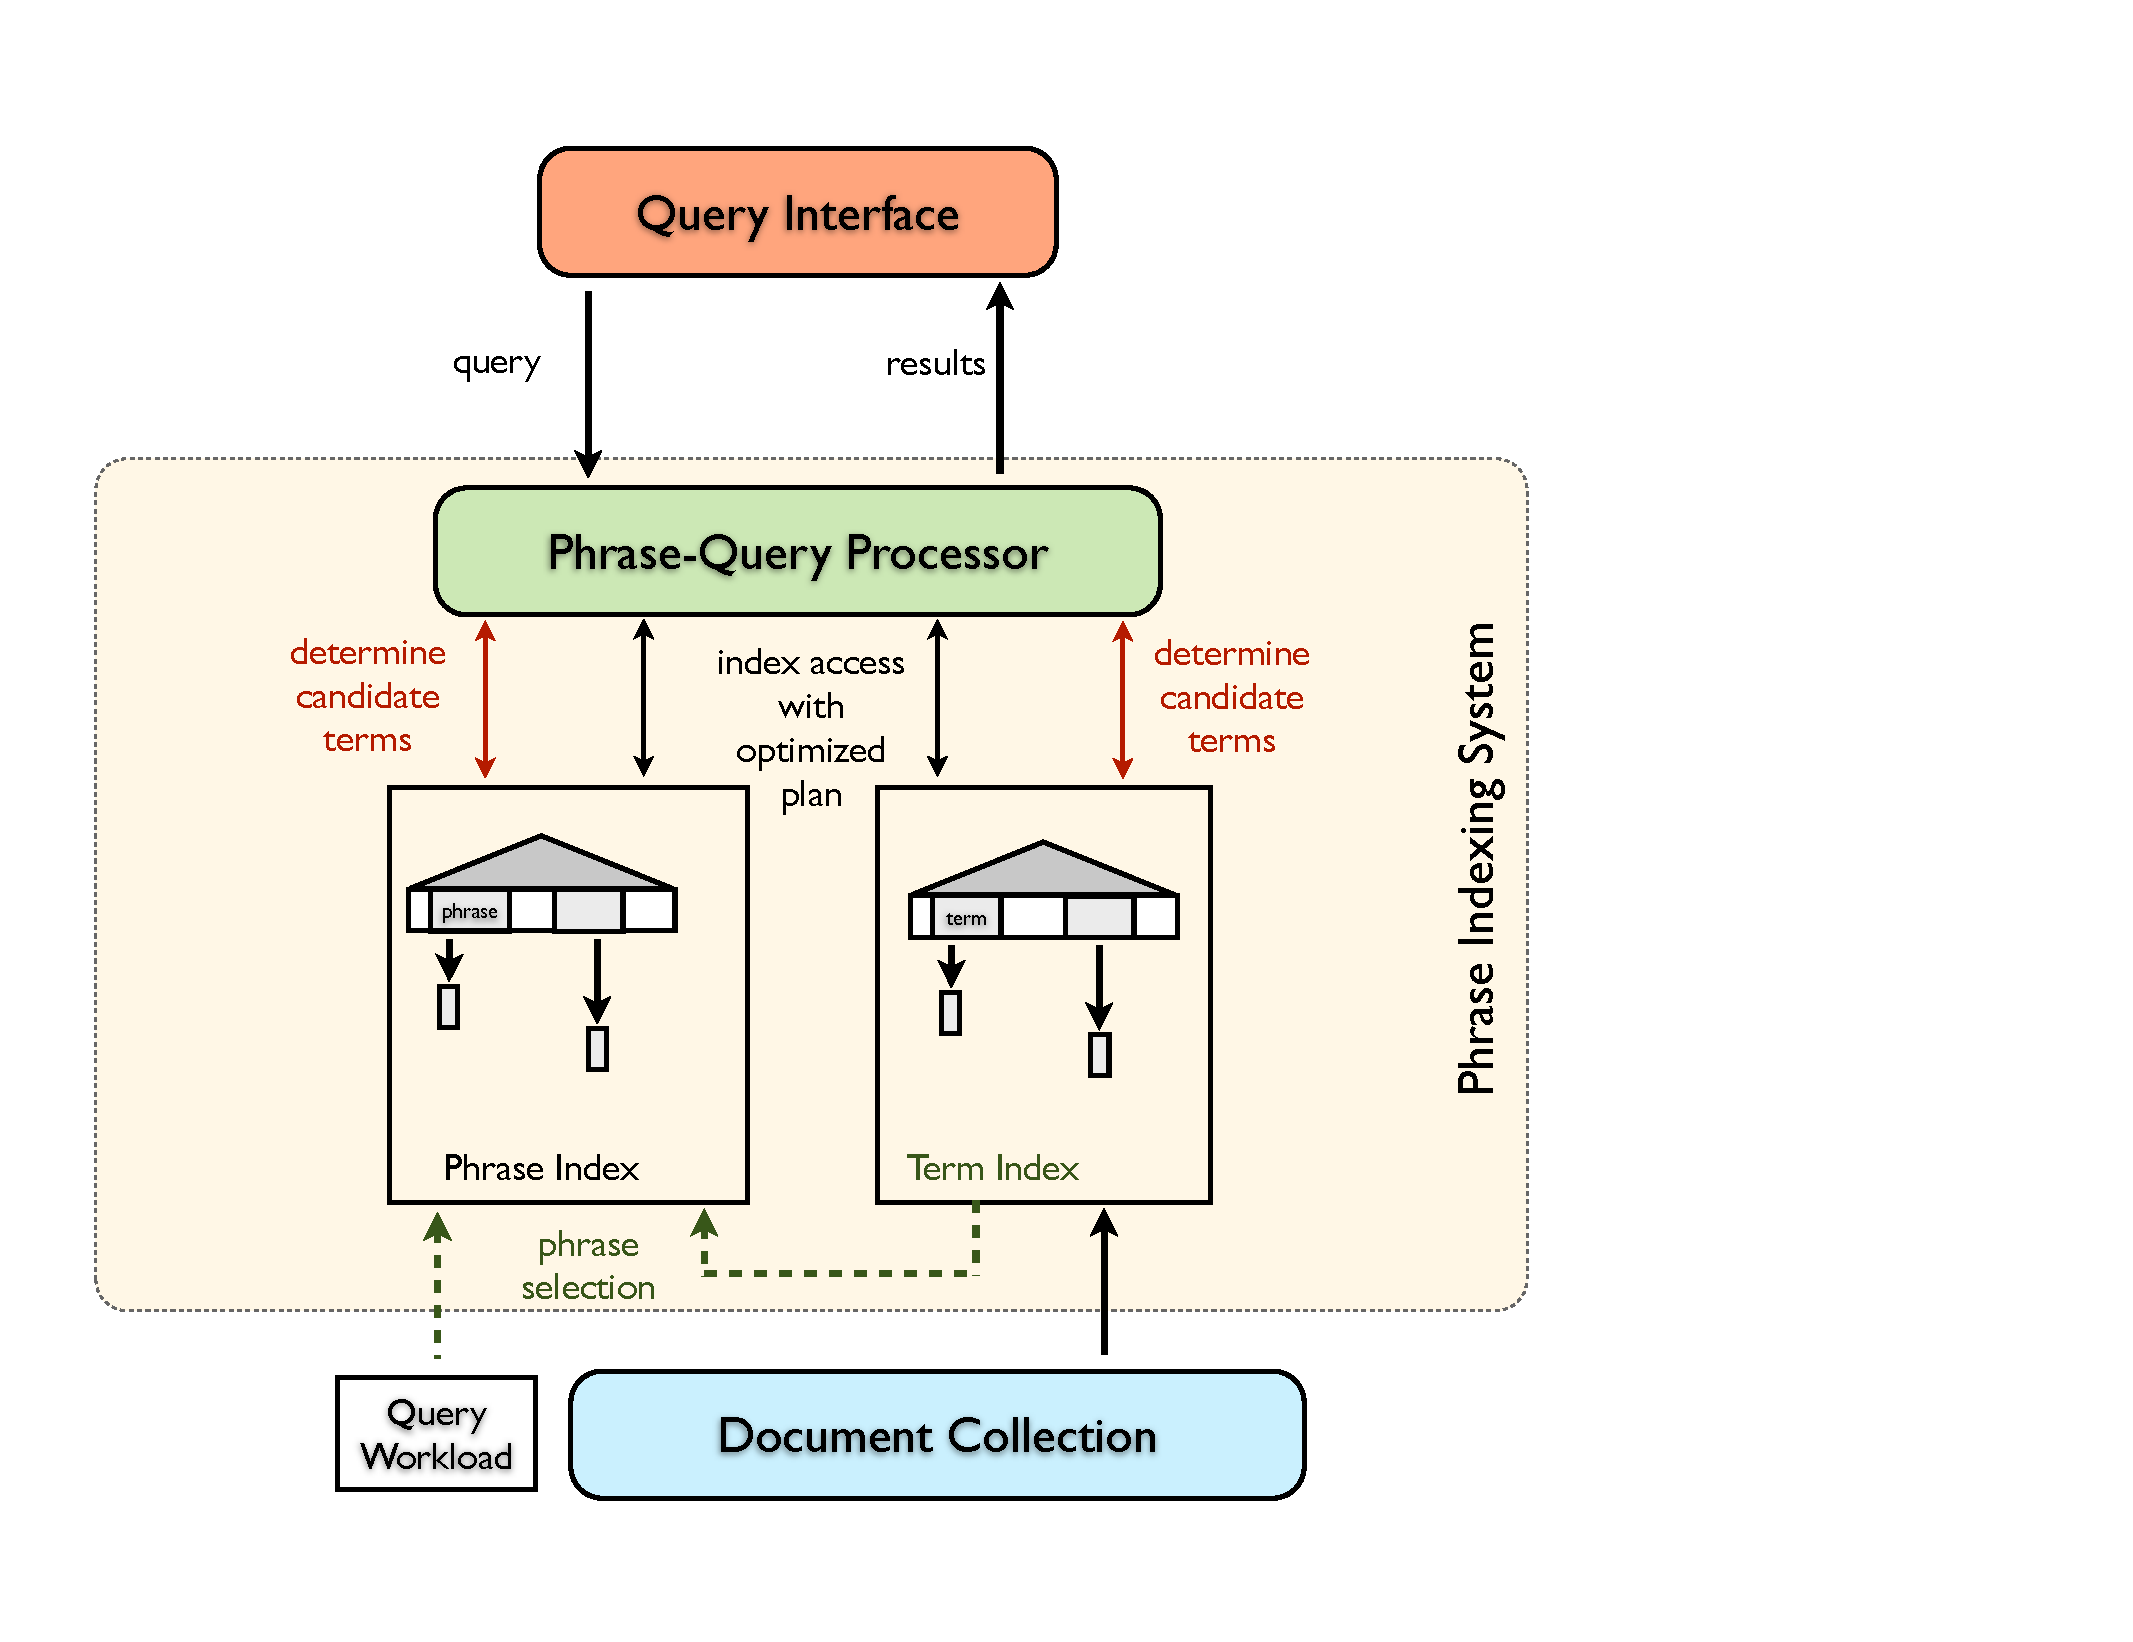
\includegraphics[width=0.85\columnwidth]{resources/epiq-sysarch.pdf}
  \caption{System architecture} 
    \label{fig:epiq_sysarch}
\end{figure}

Figure~\ref{fig:epiq_sysarch} shows a high-level overview of the architecture of our phrase-indexing system. It consists of two indexes -- the \emph{term index} and the \emph{multi-word index}. 

\begin{itemize}

\item \textbf{Term Index} It is the standard word-level inverted index consisting of the lexicon and the inverted files built over the document collection. It indexes all single words with their positional information.

\item \textbf{Phrase Index} It is constructed over the document collection for a set of phrases selected employing the phrase-selection algorithms detailed in Section~\ref{sec:phrase-selection}.

\end{itemize}

In practice, we build the term index first and its associated lexicon. The statistics required for the phrase-selection algorithm are computed from the lexicon and the query workload. The selection algorithms are then executed and a \emph{selection set} of word-sequences are determined which have to be indexed in the phrase index.
Typically, the selected set is small in size and fits in memory. Hence, indexing infrastructure for indexing words can be reused employing the selection set of word sequences to filter out sequences which do not need to be indexed. 

While processing queries, both the lexicons, for term and the phrase index, are consulted to determine the candidate words or word sequences presented in the query. Query optimization is performed over the candidate terms to determine the best plan. Finally, the respective indexes are accessed, for the terms in the optimized plan, for fetching and intersecting the posting lists to compute results.

\section{Experimental Evaluation}
\label{sec:exper-eval}

In this section, we describe our experimental evaluation. We begin
with details about our experimental setup including employed datasets,
before describing our comparison of the query-optimization methods
from Section~\ref{sec:query-optimization}, followed by an evaluation
of our phrase-selection methods from
Section~\ref{sec:phrase-selection} against state-of-the-art
competitors.

\subsection{Setup}
All indexes were built on a local Hadoop cluster
consisting of ten Dell R410 server-class computers, each equipped with
64 GB of main memory, two Intel Xeon X5650 6-core CPUs, and four
internal 2 TB SAS 7,200 rpm hard disks configured as a
bunch-of-disks. The machines are connected by 10~Gbit Ethernet, run
Cloudera CDH3u0 as a distribution of Hadoop 0.20.2, and use Oracle
Java 1.6.0\_26. Query optimization and phrase-selection experiments
were performed on a Dell PowerEdge M610 server with 2 Intel Xeon E5530
CPUs, 48 GB of main memory, a large iSCSI-attached disk array, Debian
GNU/Linux (SMP Kernel 2.6.29.3.1) and running Oracle Java
1.6.0\_34. Wall-clock time measurements were performed with the Java
Hotspot 64-Bit Server VM using the CMS garbage collector.


\subsection{Datasets Used} We use two real-world document
collections for our experiments:
\begin{itemize}

\item \emph{ClueWeb09-B}~\cite{cw} (\textsc{CW}) -- ClueWeb09-B is a subset of the ClueWeb09 corpus consisting of more than 50
  million web documents in English language crawled in 2009; 

\item \emph{The New York Times Annotated Corpus}~\cite{NYT}
  (\textsc{NYT}) -- The New York Times Annotated Corpus, as introduced in the previous chapter, contains more than 1.8 million newspaper articles published
  by The New York Times between 1987 and 2007.

\end{itemize}
Both document collections were processed using Stanford
CoreNLP~\cite{corenlp} for tokenization. To make CW more handleable,
we use boilerplate detection as described
in~\cite{Kohlschutter:2010fk} and available in the
\texttt{DefaultExtractor} of boilerpipe~\cite{boilerpipe} .

\subsection{Query Workload} As a workload we use entity labels from the YAGO2
knowledge base~\cite{Hoffart:2013fk}. In its \texttt{rdfs:label}
(formerly \texttt{means}) relation, YAGO2 collects strings that may
refer to a specific entity, which are mined from anchor texts in
Wikipedia. For the entity \texttt{Bob\_Dylan}, as a concrete example,
it includes among others the entity labels \textsf{``bob dylan''},
\textsf{``bob allen zimmerman''}, and \textsf{``robert allen
  zimmerman''}. In total, the workload that we obtain contains $13.4$
million entity labels having an average length of $2.41$
words. Interestingly, almost $99\%$ of them do not contain any
repeated word; we observe at most eight repeated words for the phrase
queries in our workload. We only consider those entity labels for
which all constituent words occur in the document collection at hand,
leaving us with $10.7$ million and $8.0$ million phrase queries for CW
and NYT, respectively. 

For our experiments on the query-optimizers effectiveness, we additionally consider a subset of our workload which refer to artist names, albums and song titles. Some examples of phrases in this workload are \textsf{``american national anthem''}, \textsf{``and the green grass grew all around''} etc. The workload that we obtain has $107,245$ entity labels having an average length of $3.4$ words. 


%To examine the effect of the query optimizer of longer query lengths we additionally considered a subset of our workload which refer to artist names, albums and song titles. 

\subsection{Index Management and Competitors} 

We implemented our indexing framework
using Hadoop. The lexicon, containing for each term its term
identifier, document frequency, and collection frequency, is stored in
a flat file and loaded into main memory at runtime. Posting lists are
kept in an indexed file (implemented using Hadoop's \texttt{MapFile})
and are stored using variable-byte encoding in combination with d-gaps
for document identifiers of consecutive postings and offsets within
each posting. We use \textsc{TaaT} to process phrase queries.

We compare against the following methods in our
experiments -- some from the literature and others conceivable
baselines:
\begin{itemize}

\item{\textbf{Uni-Gram Index}} (UNI) indexes unigrams and does not
  select any phrases;

\item{\textbf{Oracle Index}} (ORA) indexes unigrams and selects all
  phrase queries from the workload as phrases;

\item{\textbf{Next-Word Index}}~\cite{Williams:2004fk} (NEXT) indexes
  unigrams and selects all bigrams from the workload that contain a
  stopword as phrases;

\item{\textbf{Combined Index}}~\cite{Williams:2004fk} (COMB) combines
  NEXT and ORA. In the original paper, the authors considered, instead
  of ORA, a phrase index that contains precomputed results of popular
  phrase queries. ORA thus selects a superset of the phrases that the
  original approach considered. We further strengthen this competitor,
  in comparison to its original description, by using phrases from ORA
  also to process other longer phrase queries. Thus, if
  \textsf{``united states''} has been selected by ORA, our query
  optimizer may use it to processing the phrase query
  \textsf{``president of the united states''}.

\item{\textbf{Bi-Gram Index}} (BI) indexes unigrams and selects
  all bigrams from the workload as phrases;

\item{\textbf{Tri-Gram Index}} (TRI) indexes unigrams and selects all
  bigrams and trigrams from the workload as phrases;

\item{\textbf{Out-of-Box Index}}~\cite{Transier:2008kx} (OOBI) indexes
  unigrams and selects all bigrams whose cost is above a
  user-specified threshold. Unlike the other competitors, OOBI is thus
  also \emph{tunable}. To make it comparable to our phrase-selection
  methods, we adapt it, so that it ranks bigrams in descending order
  of their document frequency and selects phrases from the obtained
  list until the user-specified space budget has been exhausted.

\end{itemize}

We compare these approaches against our query-optimizer-based
selection (QOBS) and coverage-based selection (CBS). We use document
frequency as a cost measure for all our experiments. As mentioned
earlier, one could use collection frequency instead. In practice,
though, the two measures are highly correlated and we did not observe
big differences. Also, as a one-time pre-processing performed using
Hadoop and made available to all methods, we computed document
frequencies in the workload and the document collection for all
$n$-grams from the entire workload.

\begin{table*}\centering \footnotesize
\begin{tabular}{@{}llrrrcrrr@{}}\toprule
& & \multicolumn{3}{c}{\textbf{GRD}} & \phantom{abc} & \multicolumn{3}{c}{\textbf{APX}}\\ 
\cmidrule{3-5} \cmidrule{7-9}
& & $l=2$ & $l=4$ & $l=6$ && $l=2$ & $l=4$ & $l=6$\\ \midrule
&\textbf{\%}\\
\textbf{NYT}& $[0]$  & 7,586,656 & 7,839,328 & 7,877,367 && 7,662,566 & 7,868,885 & 7,900,573\\
& $(0-20)$ & 403,399 & 200,017 & 174,744 && 382,428 & 192,417 & 166,658\\
& $[20-40)$ & 70,852 & 31,399 & 22,281 && 35,157& 18, 750 & 12,712\\
& $[40-60)$ &  19,256& 9,368 & 5,706 && 12 & 111& 220\\ 
& $[60-80)$ & - & 51 & 65 && - & - & -\\
\midrule
&\textbf{\%}\\
\textbf{CW}& $[0]$ & 10,080,400 & 10,488,737 & 10,589,685  && 10,176,979 & 10,523,862 & 10,607,792\\
& $(0-20)$ & 547,289 & 204,716 & 135,579 && 525,781 & 27,894 & 132,417\\
& $[20-40)$ & 98,391 & 45,313 & 21,526 && 49,995& 27,894& 12,496\\
& $[40-60)$ & 26,700 & 13,740 & 5,764 && 25 & 136 & 75\\ 
& $[60-80)$ & - & 274 & 226 && - & - & -\\
\bottomrule
\end{tabular}
\caption{Percentage improvement in query-processing cost by OPT over GRD and APX}

\label{tab:optimizers}
\end{table*}

\begin{table*}\centering \footnotesize
\begin{tabular}{@{}llrrrcrrr@{}}\toprule
& & \multicolumn{3}{c}{\textbf{GRD}} & \phantom{abc} & \multicolumn{3}{c}{\textbf{APX}}\\ 
\cmidrule{3-5} \cmidrule{7-9}
& & $l=2$ & $l=4$ & $l=6$ && $l=2$ & $l=4$ & $l=6$\\ \midrule
&\textbf{\%}\\
\textbf{NYT}& $[0]$ & 77,130 & 82,058 & 83,708 && 79,459 & 82,703 & 84,031\\
& $(0-20)$ & 7,705 & 3,686 & 2,747 && 6,656  & 3,654 & 2,667\\
& $[20-40)$ & 1,735 & 950 & 379 && 839 & 594 & 254 \\
& $[40-60)$ & 387 & 261 & 117 && 3 & 6 & 5\\ 
& $[60-80)$ & - & 2 & 6 && - & - & - \\
\midrule

&\textbf{\%}\\
\textbf{CW}& $[0]$ & 84,108 & 91,039 & 94,839 && 86,281 & 92,034 & 95,218 \\
& $(0-20)$ & 9,888 & 4,129 & 1,849 && 9,772 & 4,259 & 1,832\\
& $[20-40)$ & 2,710 & 1,753 & 505 && 1,342 & 1,105 & 347 \\
& $[40-60)$ & 704 & 480 & 197 && 15 & 12 & 13 \\
& $[60-80)$ & - & 9 & 20 && - & - & -\\
\bottomrule
\end{tabular}
\caption{Percentage improvement in query-processing cost by OPT over GRD and APX -- on song titles}

\label{tab:songs_optimizers}
\end{table*}

\subsection{Performance of Query Optimization}

Our first experiment examines the effect that the choice of
query-optimization method can have on query-processing performance. We
consider three query-optimization methods for this experiment: the
greedy algorithm (GRD) from~\cite{Williams:2004fk}, our greedy
algorithm (APX) that gives an approximation guarantee, and our
exponential exact algorithm (OPT). GRD considers terms in increasing
order of their document frequency, thus based on their selectivity,
and chooses a term if it covers any yet-uncovered portion of the
phrase query. Originally designed to deal with bigrams only, we extend
GRD to break ties based on term length, and thus favor the longer
term, if two terms have the same document frequency.

To compare the three query-optimization methods, we built augmented
inverted indexes whose dictionaries include all phrases up to a
specific maximum length $l \in \bigset{2, 4, 6}$. Thus, for $l=4$, all
phrases of length four or less are indexed. This allows us to study
the behavior of the methods as more terms to choose from become
available.

First, we examine the different methods in terms of their runtime in
practice. We observe an average runtime of $0.01$~ms for each of them,
showing that there is no difference in practice. The maximum runtime
observed for OPT for any of the phrase queries from our workload is
$2.00$~ms, indicating that its exponential nature rarely affects its
runtime in practice. Thus, for all further experiments we use OPT as a
query-optimization method.

Second, we compare the different methods in term of the costs of their
generated query plans. To this end, we determine for each phrase query
from the workload the percentage improvement over GRD and APX,
respectively that one can achieve by using OPT. Let $C_{OPT}$,
$C_{GRD}$, and $C_{APX}$ denote the cost of the query plan (in terms
of total number of postings read) determined by the respective
query-optimization method. The percentage improvement is given by the
values $(C_{GRD} - C_{OPT})/(C_{GRD})$ and
$(C_{APX} - C_{OPT})/(C_{APX})$ that range in
$[0,1)$. Table~\ref{tab:optimizers} gives bucketed percentage
improvements for our two datasets and three augmented inverted
indexes. Each cell reports the number of phrase queries from the
workload for which a percentage improvement in the given range was
observed.

From Table~\ref{tab:optimizers}, we observe that, for the majority of phrase queries,
there is no substantial improvement (i.e., less than $20\%$) when
using OPT instead one of the non-optimal methods. Further, we see that
the number of phrase queries for which an improvement is achieved is
generally lower for APX than for GRD, which is expected given the
former's approximation guarantee. As can also be seen from the table,
there is a non-negligible number of phrase queries for which OPT
improves by $40\%$ or more over GRD. For the query \textsf{``we are
  the champions''} with $l=2$, as a concrete example, GRD picks
$\bigset{\mbox{\textsf{we are}, \textsf{are the}, \textsf{the
      champions}}}$
as a query plan, which is more than twice as expensive as the query
plan $\bigset{\mbox{\textsf{we are}, \textsf{the champions}}}$
determined by OPT. When comparing percentage improvements across
different augmented inverted indexes, we see less improvement for
larger values of $l$, which makes sense since those include longer,
more selective phrases favored by the non-optimal methods.

%To examine the effect of the query optimizer of longer query lengths we additionally considered a subset of our workload which refer to artist names, albums and song titles. Some examples of phrases in this workload are \textsf{``american national anthem''}, \textsf{``and the green grass grew all around''} etc. 

To examine the effect of the query optimizer of longer query lengths, we now look at the results on experiments on song titles summarized in Table~\ref{tab:songs_optimizers}. We observe that, like in the previous table, for majority of the queries, OPT shows no improvement over GRD and APX. However, OPT shows non-zero improvement for around 11\% of the queries in Table~\ref{tab:songs_optimizers}, as compared to the entire workload where the improvements are for less than 6\% of the queries. This means that OPT improves over the other optimizers for longer query lengths. Consistent with the previous observation, we see that APX performs better than GRD in majority of the scenarios. It is also interesting to note that, although the improvements for larger values of $l$ is lesser, the magnitude of improvement is larger as compared to $l=2,4$. As an example, for $l=6$ in CW, we see an 60\%-80\% improvements over GRD when using OPT in some queries.


In summary, neither GRD nor APX falls far behind OPT in terms of the
cost of its generated query plans. APX is robust, comes with an
approximation guarantee, and is easy to implement. However, as stated
above, we did not see any phrase query for which OPT was too expensive
to run, making it a viable choice in practice.

\begin{figure*}[!ht]
    \centering  
      \subfigure[NYT] {\label{fig:acm_nyt_nocp}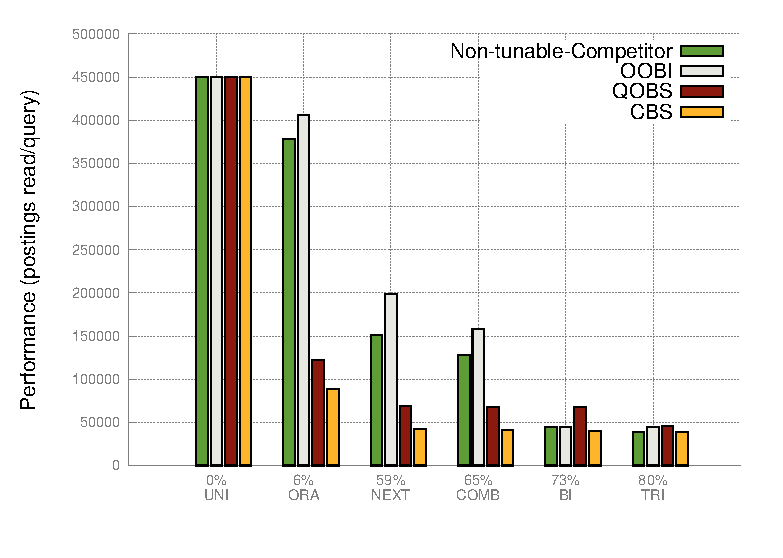
\includegraphics[width=0.8\textwidth]{plots/phrases/pdfs/nyt-acm-comp-nocp.eps}}
    \quad
    \subfigure[CW]{\label{fig:acm_cw_nocp}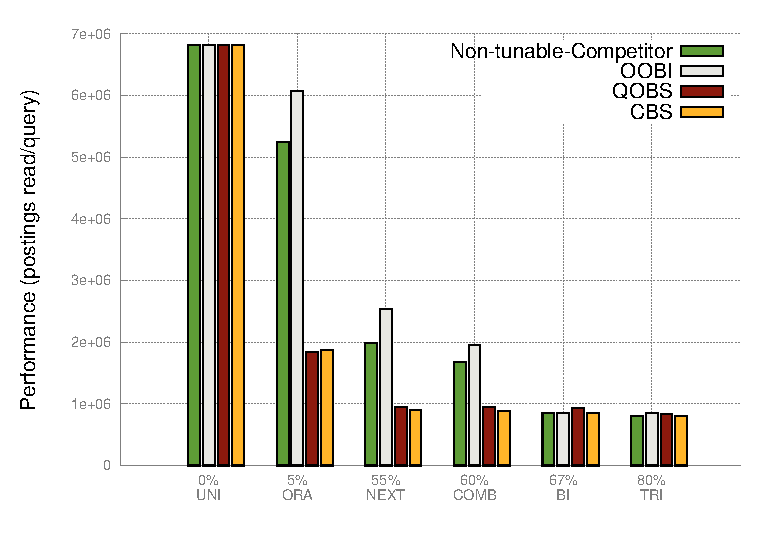
\includegraphics[width=0.8\textwidth]{plots/phrases/pdfs/cw-acm-comp-nocp.eps}}
    
    \caption{Performance of tunable phrase-selection methods relative to non-tunable competitors in terms of abstract cost measures}
    
    \label{fig:non-tunable}
\end{figure*}

  \begin{figure*}[!ht]
  \centering  
    \subfigure[NYT] {\label{fig:wct_nyt}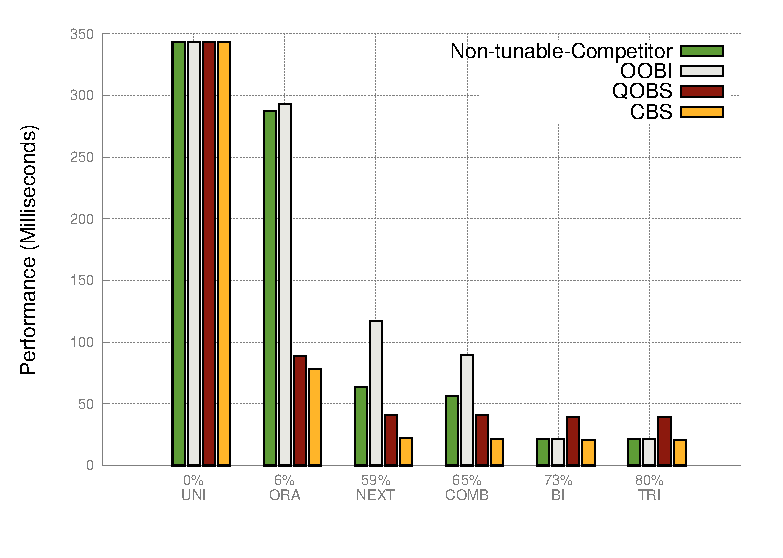
\includegraphics[width=0.8\textwidth]{plots/phrases/pdfs/nyt-wct-nocp.eps}}
    \quad
    \subfigure[CW]{\label{fig:wct_cw}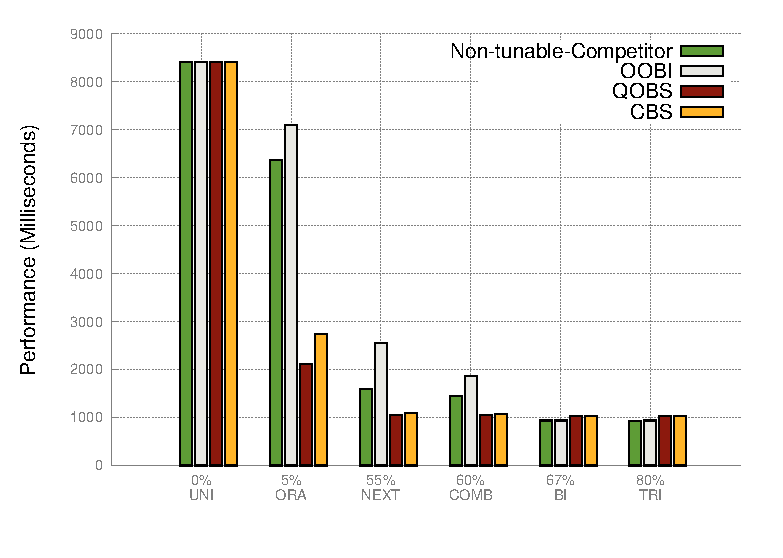
\includegraphics[width=0.8\textwidth]{plots/phrases/pdfs/cw-wct-nocp.eps}}
    
    \caption{Performance of tunable phrase-selection methods relative to non-tunable competitors in terms of wall-clock times}
    
    \label{fig:non-tunable}
\end{figure*}

\begin{figure*}[!ht]
    \centering  
      \subfigure[NYT] {\label{fig:acm_nyt_nocp}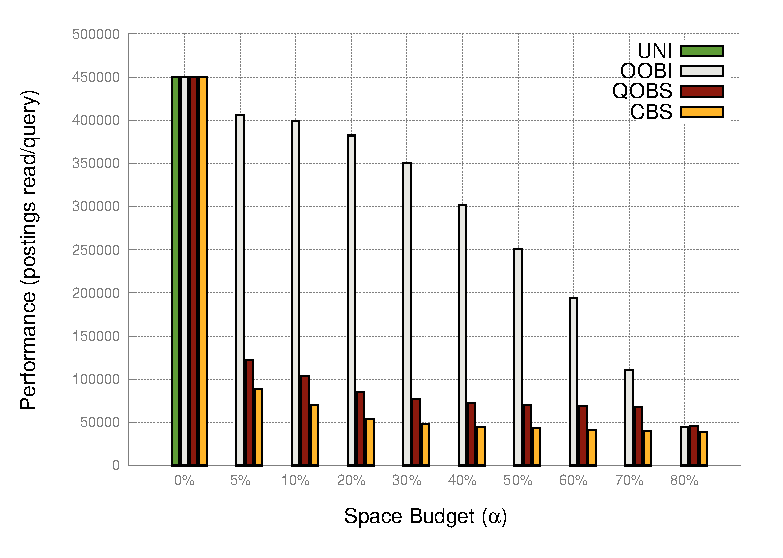
\includegraphics[width=0.8\textwidth]{plots/phrases/pdfs/nyt-acm-nocp.eps}}
    \quad
    \subfigure[CW]{\label{fig:acm_cw_nocp}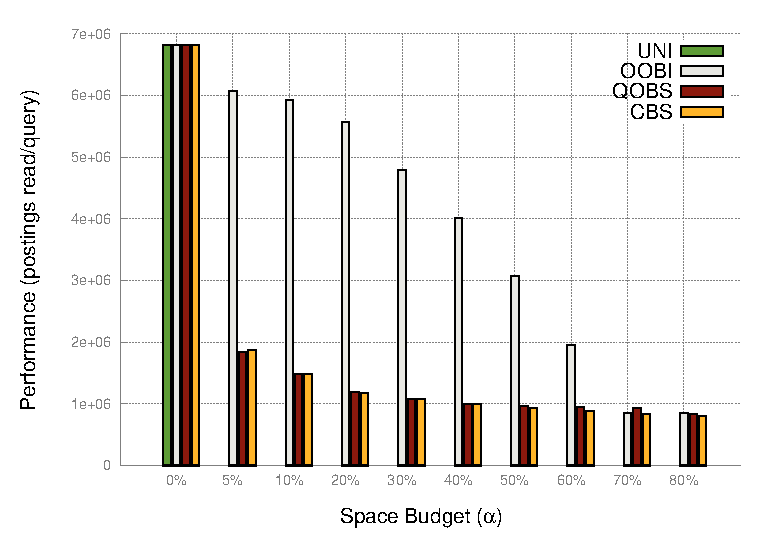
\includegraphics[width=0.8\textwidth]{plots/phrases/pdfs/cw-acm-nocp.eps}}
    
    \caption{Performance of tunable phrase-selection methods}
    
    \label{fig:tunable}
\end{figure*}

\subsection{Effect of Phrase Selection}

Our second experiment compares our phrase-selection methods against
their tunable and non-tunable competitors in terms of query-processing
performance.

We use five-fold cross validation throughout this experiment. Our
workload is split into five folds, yielding five training-test
configurations. Phrase selection is then performed using the four
training folds; query-performance measurements are performed using the
test fold. We report averages over the five training-test
configurations.

For all methods, we assume that single words are present in the
lexicon -- UNI thus serves as a baseline that all methods under
comparison build upon. On CW the standard positional inverted index
obtained by UNI amounts to $71$~GB and contains a total of $90.17$
billion postings; on NYT the corresponding index amounts to $3$~GB and
contains a total of $4.91$ billion postings. Index sizes, in the
following, are indicated in terms of their percentage overhead over
UNI -- an index size of $10\%$ thus means that the corresponding is
$1.1\times$ larger than the baseline index.

Query-processing performance is measured both in abstract and concrete
terms. As an abstract cost measure, we use the average number of
postings that is read to process a phrase query from the test
folds. We use wall-clock times (in milliseconds) as a concrete cost
measure. These were obtained based on a sample of $25,000$ phrase
queries ($5,000$ per test fold), using a single core, and pre-fetching
all required posting lists into main memory. 

Figure~\ref{fig:non-tunable} compares the tunable phrase-selection
methods (QOBS, CBS, OOBI) against their non-tunable competitors. As a
first step, we built an index for each of the non-tunable
competitors. The sizes of these indexes determine the values of
$\alpha$, which we feed into the tunable phrase-selection methods to
obtain indexes of correspond sizes, in a second step. For the sake of
comparison, we include UNI in Figure~\ref{fig:non-tunable},
corresponding to $\alpha = 0$, that is, no phrases are selected.

We observe that ORA results in the smallest index, since it
materializes only phrases that occur in exactly that form as phrase
queries in the workload. However, doing so, it overfits to the
training folds, resulting in query-processing performance that is only
slightly better than our baseline UNI. When given the same amount of
additional space ($6\%$ for NYT and $5\%$ for CW), our tunable
phrase-selection methods QOBS and CBS achieve considerably better
query-processing performance -- an improvement by at least a factor
$3\times$ over ORA and the baseline UNI in terms of both abstract and
concrete measures. NEXT and COMB, materializing all bigrams from the
training folds that contain a stopword, result in indexes that consume
$55\%-60\%$ additional space. While they achieve good improvements in
query-processing performance over the baseline, they are consistently
outperformed by QOBS and CBS. BI and TRI, which result in indexes that
require $67\%-80\%$ of additional space, improve query-processing
performance by at least a factor $7\times$ over the baseline. From the
tunable phrase-selection methods OOBI and CBS perform at par, when
given this much additional space. While this also holds for QOBS on
CW, it performs slightly worse than its competition on NYT. Moreover,
we see that the trends observed in abstract and concrete measures of
query-processing performance are consistent. In the rest of this
section, we thus only consider abstract cost measures.

Figure~\ref{fig:tunable} compares our tunable phrase-selection methods
QOBS and CBS against OOBI as the only tunable competitor. For all
three methods, we constructed indexes considering values of $\alpha$
ranging from $5\%$ to $80\%$. UNI is again included at $\alpha=0\%$
for the sake of comparison. With as little as $5\%$ additional space,
QOBS and CBS improve query-processing performance by at least a factor
$3\times$. When comparing our two methods, we observe that CBS
performs slightly better than QOBS on NYT, whereas their performance
is comparable on CW. QOBS and CBS perform consistently better than
their sole competitor OOBI. When given $5\%$ additional space, as a
concrete figure, OOBI improves over UNI by at most a factor
$1.2\times$. What is also apparent from the figure are the diminishing
returns of additional space, which are more pronounced for our methods
that already make highly effective use of the initial $5\%$ of
additional space. Finally, when given ample additional space, all
tunable phrase-selection methods perform at par.

% \subsection{Robustness of Phrase Selection}
% %experimental setup
% To test robustness of our tunable selection methods we considered increasing sizes of training sets of queries and tested on a fixed test set. We cumulatively increased the training sample adding 10\% more queries in each round. We plot the performance in terms of postings read per query in y-axis of Figure~\ref{fig:rob} and the training size as a fraction of the entire training set on the x-axis. We consider all the three tunable approaches with 3 size budget parameters of 1\%, 10\% and 100\% of TERM. 

% We observe that for a smaller size budgets(1\% and 10\%) OOBI is very robust, although with inferior overall performance. This is due to the fact that OOBI selects often repeated phrases like ``of the'', ``in the'' which have a higher occurence frequency in the collection and fills up its allocated space budget. An increase in training data sizes is ineffective to this extent. Our approaches are judicious in selection of phrases taking into account the occurence frequencies in the workload to optimize query performance and with indeed show an improvement in performance with the increase in workload size. However, the overall performance is reasonably stable with a overall performance difference of less than 17\%(NYT) and XXX(CW) between 20\% and 100\% of training data for both CBS and QOBS. When we have no limits on the size budget (budget parameter - 1.0), all the methods seem to have same trends. In fact, the performance of all methods are highly correlated. Even then the improvement in performance flattens out after 40\% of the training set has been considered.
% %robustness statement

% \begin{figure*}[ht] 
%     \centering  
%       \subfigure[NYT] {\label{fig:rob_nyt_nocp}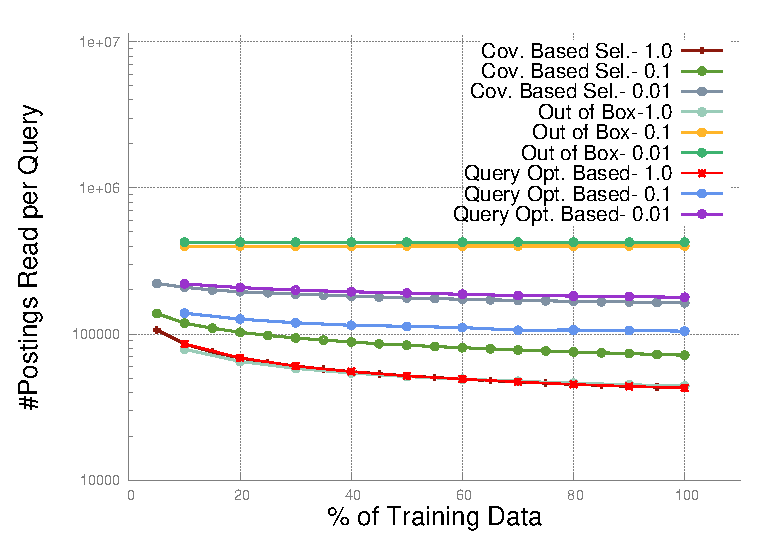
\includegraphics[width=0.4\textwidth]{plots/phrases/pdfs/nyt-rob.eps}}
%     \quad
%     \subfigure[CW]{\label{fig:rob_cw_nocp}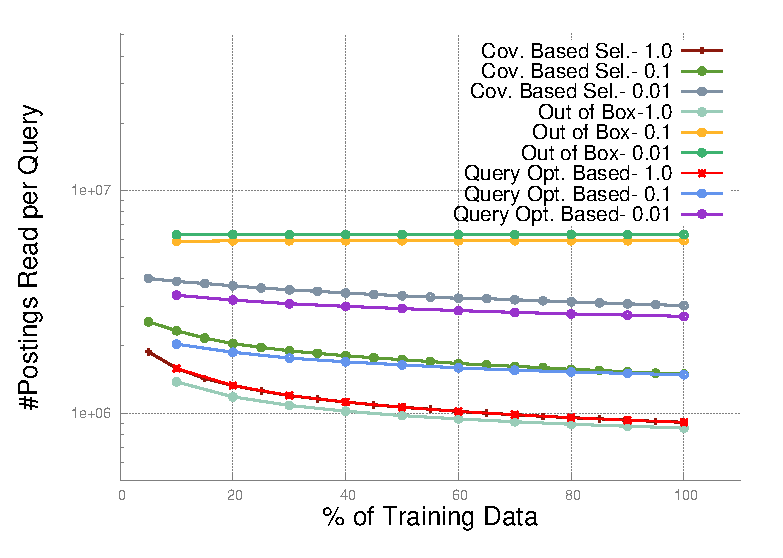
\includegraphics[width=0.4\textwidth]{plots/phrases/pdfs/cw-rob.eps}}
    
%     \caption{Robustness of phrase-selection methods}
    
%     \label{fig:tunable}
% \end{figure*}

\section{Related Work}
\label{sec:related-work}

We now discuss the connection between our work and existing prior
work, which we categorize as follows:

\textbf{Phrase Queries.} Williams et al.~\cite{Williams:2004fk} put
forward the \emph{combined index} to support phrase queries
efficiently. It assembles three levels of indexing: (i)~a
\emph{first-word index} as a positional inverted index, (ii)~a
\emph{next-word index} that indexes all bigrams containing a stopword,
and (iii)~a \emph{phrase index} with popular phrases from a query
log. Its in-memory lexicon is kept compact by exploiting common
first words between bigrams. Query processing escalates through these
indexes -- first it consults the phrase index and, if the phrase query
is not found therein, processes it using bigrams and unigrams from the
other indexes. Transier and Sanders~\cite{Transier:2008kx} select
bigrams to index based only on characteristics of the document
collection. Selecting bigrams makes sense in settings where phrase
queries are issued by human users and tend to be short -- as observed
for web search by Spink et al.~\cite{Spink:2001}. We also target
application-generated queries (e.g., quotations and titles of movies
or songs) and thus select variable-length phrases. Those have
previously been considered by Chang and Poon~\cite{Chang:2008kx} in
their \emph{common phrase index}, which builds
on~\cite{Williams:2004fk}, but indexes variable-length phrases common
in the workload. Our methods, in contrast, consider both the document
collection and the workload.

\textbf{Proximity} scoring, such as the model by B\"uttcher
et al.~\cite{Buttcher:2006kx}, is similar in spirit to phrase queries
but targets ranked retrieval. Proximity of query words is an important
signal in modern web search engines. Several authors have looked into
making the computation of proximity scores more efficient. Yan et
al.~\cite{Yan:2010tw} propose a word-pair index and develop
query-processing methods that support early termination. Broschart and
Schenkel~\cite{BroschartS12} describe a tunable word-pair index that
relies on index pruning to keep its size manageable. Fontoura et
al.~\cite{Fontoura:2011uq} describe an alternative method of indexing
word pairs, which maintains them as bitmaps along with posting lists
for single words.

\textbf{Caching} is often used to speed up query processing and reduce
the overall system load. It can be applied at different granularities
including query results, posting lists of single words, and
posting-list intersections. The first two are considered by Saraiva et
al.~\cite{Saraiva:2001} as well as Baeza Yates et
al.~\cite{baeza2008design}. Long and Suel~\cite{Long:2006fk}
propose a three-level cache that also includes posting-list
intersections. Going beyond that, Ozcan et al.~\cite{Ozcan:2012fk}
describe a five-level cache that additionally includes result snippets
and documents. Policies for admitting/evicting items to/from the cache
have been described, among others, by Baeza-Yates et
al.~\cite{Baeza-Yates:2007adm} as well as Gan and
Suel~\cite{Gan:2009}. Fagni et al.~\cite{Fagni:2006} distinguish
between a static and a dynamic cache, where the former is periodically
bootstrapped from query logs, and the latter is managed using a
replacement policy such as LRU. While none of the aforementioned works
has specifically addressed phrase queries, it is conceivable to add a
layer that caches phrases as intersections of multiple posting
lists. Our phrase-selection methods could then be used to bootstrap a
(static) cache.

\section{Summary}
~\label{chap:phrases:sec:conclusion}

In this chapter we developed efficient solution to processing phrase queries. We studied how arbitrary phrase queries can be efficiently processed over an augmented-inverted index of word sequences. We developed methods to select multi-word sequences to be indexed to optimize query-processing cost while keeping the index size within a user-specified budget. We also proposed novel query-optimization techniques to efficiently process phrase queries over such an augmented index.

With regard to phrase-query optimization, a first
insight from our experiments is that the non-optimal methods perform
close to the optimum for a majority of phrase queries. As a second
insight, we observed that our tunable phrase-selection methods make
highly effective use of additional space, in particular when there is
only little of it, and considerably improve the processing performance
of phrase queries.
